\begin{flushright} {\tiny {\color{gray} \tt fdm\_stokes2D.tex}} \end{flushright}
%~~~~~~~~~~~~~~~~~~~~~~~~~~~~~~~~~~~~~~~~~~~~~~~~~~~~~~~~~~~~~~~~~~~~~~~~~~~~~~~~~~~~~~~~~~~~~~~~~~

%---------------------------------------------------------
\subsection{A quick recap of the incompressible 2D Stokes equations}

In the case of an incompressible and isoviscous flow, we can start  from the momentum equation
\begin{equation}
-\vec\nabla p + \vec\nabla \cdot {\bm \tau} + \rho \vec{g} = \vec{0}
\end{equation}
with\footnote{Since the flow is incompressible we will not distinguish
between the strain rate tensor and the deviatoric strain rate tensor 
since they are identical.} 
\begin{equation}
{\bm \tau} = 2 \eta \dot{\bm \varepsilon}(\vec\upnu)
\end{equation}
In 2D the strain rate tensor components are given by
\[
\dot{\varepsilon}_{xx}=\frac{\partial u}{\partial x}
\quad\quad\quad
=\dot{\varepsilon}_{yx}
=\frac{1}{2} \left( \frac{\partial u}{\partial y} + \frac{\partial v}{\partial x} \right)
\quad\quad\quad
\dot{\varepsilon}_{yy}=\frac{\partial v}{\partial y}
\]
In the end we obtain the following set of coupled PDEs for the three 
unknwons $u,v,p$:
\begin{eqnarray}
-\frac{\partial p}{\partial x}  
+ 2 \frac{\partial }{\partial x} \left(\eta \frac{\partial u}{\partial x}  \right) 
+\frac{\partial}{\partial y}\left(\eta (\frac{\partial u}{\partial y}+\frac{\partial v}{\partial x}) \right)
+  \rho g_x &=&0 \\
-\frac{\partial p}{\partial y}  
+ 2 \frac{\partial }{\partial y} \left(\eta \frac{\partial v}{\partial y}  \right) 
+\frac{\partial}{\partial x}\left(\eta (\frac{\partial u}{\partial y}+\frac{\partial v}{\partial x}) \right)
+  \rho g_y  &=& 0 \\
\frac{\partial u}{\partial x} + \frac{\partial v}{\partial y}  = 0 
\end{eqnarray}

Note that in their syllabus \textcite{beka} add the term $p/\lambda$ to the rhs
of the incompressibility equation: 
\begin{displayquote}
{\color{darkgray}
This is a ``trick'' called
the penalty method, which ensures that the system of equations does not become ill-
posed. For this to work, $\lambda$ should be sufficiently large 
($\sim 10^4$ or so), so that the condition
of incompressibility is approximately satisfied.}
\end{displayquote} 


Then, {\it if the viscosity is constant} the $x$-component of 
the momentum conservation equation
\[
-\frac{\partial p}{\partial x}  
+ 2\eta \frac{\partial \dot{\varepsilon}_{xx}}{\partial x} 
+ 2\eta \frac{\partial \dot{\varepsilon}_{xy}}{\partial y}  + \rho g_x =0
\]
becomes
\[
-\frac{\partial p}{\partial x}  
+ 2\eta \frac{\partial^2 u}{\partial x^2} 
+ \eta \left( \frac{\partial^2 u}{\partial y^2 } 
+ \frac{\partial^2 v}{\partial x \partial y} \right)  \rho g_x =0
\]
Using ${\vec \nabla} \cdot {\vec v} = 0$ to obtain 
$\frac{\partial u}{\partial x} =  - \frac{\partial v}{\partial y}  $ we arrive at 
\[
-\frac{\partial p}{\partial x}  
+ \eta \left( \frac{\partial^2 u}{\partial x^2} 
+ \frac{\partial^2 u}{\partial y^2 }  \right)
+ \rho g_x =0
\]
The same approach can be carried out for the $y$-component of the momentum conservation
equation and in the end
these are the three coupled equations we need to solve
\begin{eqnarray}
-\frac{\partial p}{\partial x}  
+ \eta \left( \frac{\partial^2 u}{\partial x^2} 
+ \frac{\partial^2 u}{\partial y^2 }  \right) + \rho g_x &=&0 \\
-\frac{\partial p}{\partial y}  
+ \eta \left( \frac{\partial^2 v}{\partial x^2} 
+ \frac{\partial^2 v}{\partial y^2 }  \right) + \rho g_y  &=& 0 \\
\frac{\partial u}{\partial x} + \frac{\partial v}{\partial y}  = 0 
\end{eqnarray}
Of course these PDEs must be supplemented by appropriate boundary conditions.

At this stage we must acknowledge (as in the FEM case) that it would be pointless
to blindly discretise the equations above. Much work has been done on the topics
for decades and only certain approaches have proven succesful. 
The book of Taras Gerya (1st and second edition \cite{gery10,gery19book}) 
remains the reference in geodynamics and what follows is greatly influenced by this book. 


%--------------------------------------------
\subsection{A quick note about the MAC sheme}

The MAC scheme originates in \textcite{hawe65} (1965) and is nicely
summed up in \textcite{kans08} (2008) and \textcite{mctf08} (2008).
Before going any further we need to highlight a few points from the original paper.
First, 
\begin{displayquote}
{\color{darkgray}
One point should be emphasized. The marker particles introduced into 
this incompressible flow calculation are only for the purpose 
of indicating fluid configuration. They show which cells contain fluid
and especially which cells lie along the free surface. [...]
They do not participate in the calculation as do the Particle-in-Cell-method
particles in the Los alamos computer program for compressible flows.
}
\end{displayquote}
Second, looking at ther equations
\begin{center}
\fbox{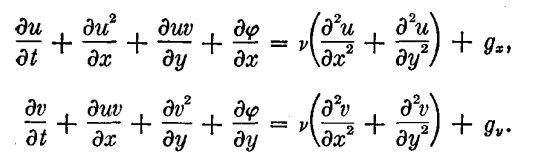
\includegraphics[width=7cm]{images/fdm/hawe65_a}}
\end{center}
we read that $\varphi$ is the ratio of the pressure to the (constant) density
and that $\nu=\eta/\rho$ is the kinematic viscosity coefficient. 
This constant-density approximation is quite limiting in the context 
of geodynamics where buoyancy-driven flow is important so 
we will not pursue this direction further. Likewise the constant-viscosity
approximation is also not desirable.

Before moving on, it is quite interesting that 
when looking at their Fig.~2, we find that the spatial 
layout of the unknowns is of the staggered type:
\begin{center}
\fbox{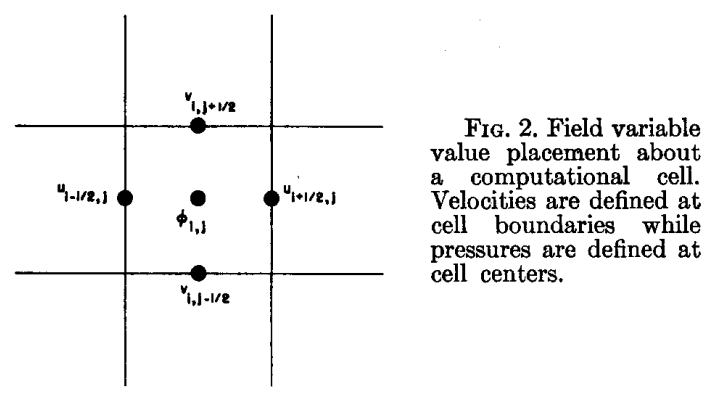
\includegraphics[width=7cm]{images/fdm/hawe65_b}}
\end{center}



%------------------------------------
\subsection{The fully staggered grid}

Let us consider a 2D Cartesian domain of size $L_x \times L_y$.
It can be shown that the following layout of nodes is necessary 
if the FDM is to be successful\footnote{In other words
any attempt where $u$, $v$, $p$ would be on the corner nodes is doomed.}:
Note that in what follows we consider a mesh where all nodes are equidistant.
This is not a requirement of the method but it allows for more compact notations
\footnote{We will revisit this topic in Section~\ref{ss:fdm_stokes_hvar}.}. 

We find a similar staggered grid figure in Gerya's book:

\begin{flushright} {\tiny {\color{gray} (tikz\_staggered2D.tex)}} \end{flushright}
%~~~~~~~~~~~~~~~~~~~~~~~~~~~~~~~~~~~~~~~~~~~~~~~~~~~~~~~~~~~~~~~~~~~~~~~~~~~~~~~~~~~~~~~~~~~~~~~~~~

\begin{center}
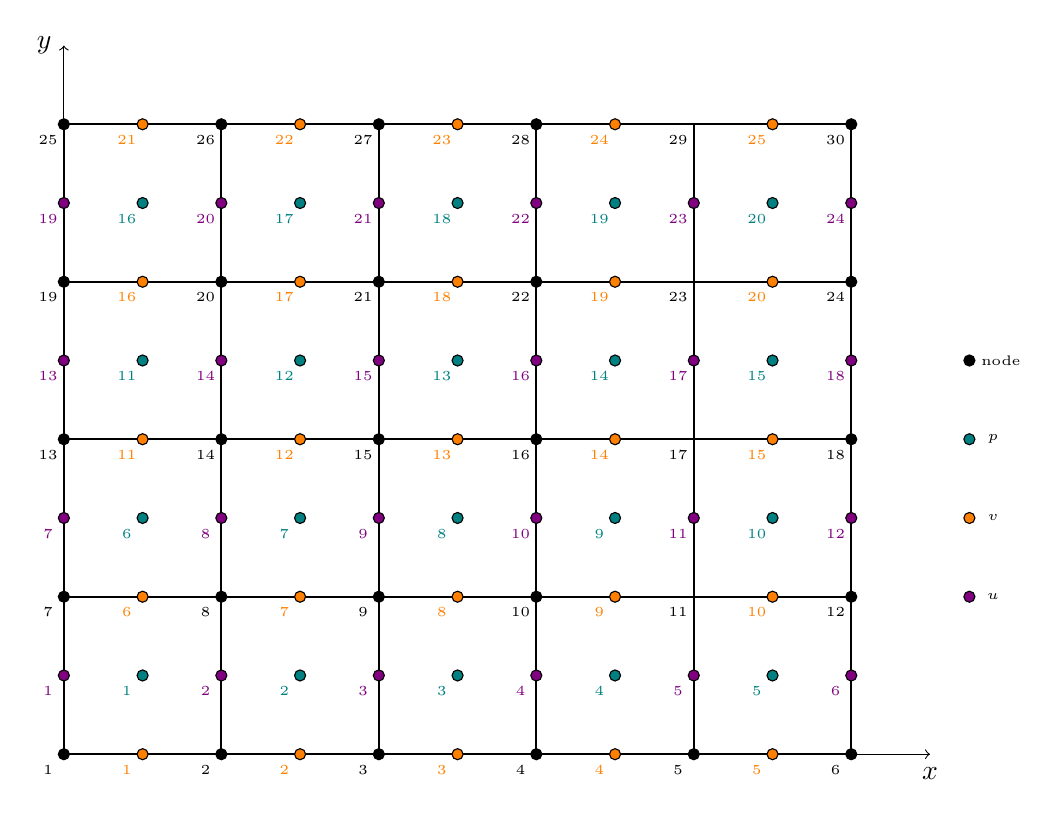
\begin{tikzpicture}
%\draw[fill=gray!23,gray!23](0,0) rectangle (12,10);
%\draw[step=0.5cm,gray,very thin] (0,0) grid (12,10); %background grid

\draw[thick] (0,0) -- (10,0) -- (10,8) -- (0,8) -- cycle ; %1-4
\draw[thick] (0,2) -- (10,2)  ; 
\draw[thick] (0,4) -- (10,4)  ; 
\draw[thick] (0,6) -- (10,6)  ; 
\draw[thick] (2,0) -- (2,8)  ; 
\draw[thick] (4,0) -- (4,8)  ; 
\draw[thick] (6,0) -- (6,8)  ; 
\draw[thick] (8,0) -- (8,8)  ; 

%pressure nodes
\draw[black,fill=teal] (1,1)   circle (2pt); %1
\draw[black,fill=teal] (3,1)   circle (2pt); %1
\draw[black,fill=teal] (5,1)   circle (2pt); %1
\draw[black,fill=teal] (7,1)   circle (2pt); %1
\draw[black,fill=teal] (9,1)   circle (2pt); %1
\draw[black,fill=teal] (1,3)   circle (2pt); %1
\draw[black,fill=teal] (3,3)   circle (2pt); %1
\draw[black,fill=teal] (5,3)   circle (2pt); %1
\draw[black,fill=teal] (7,3)   circle (2pt); %1
\draw[black,fill=teal] (9,3)   circle (2pt); %1
\draw[black,fill=teal] (1,5)   circle (2pt); %1
\draw[black,fill=teal] (3,5)   circle (2pt); %1
\draw[black,fill=teal] (5,5)   circle (2pt); %1
\draw[black,fill=teal] (7,5)   circle (2pt); %1
\draw[black,fill=teal] (9,5)   circle (2pt); %1
\draw[black,fill=teal] (1,7)   circle (2pt); %1
\draw[black,fill=teal] (3,7)   circle (2pt); %1
\draw[black,fill=teal] (5,7)   circle (2pt); %1
\draw[black,fill=teal] (7,7)   circle (2pt); %1
\draw[black,fill=teal] (9,7)   circle (2pt); %1
\node[] at (0.8,0.8) {\tiny \color{teal} 1};
\node[] at (2.8,0.8) {\tiny \color{teal} 2};
\node[] at (4.8,0.8) {\tiny \color{teal} 3};
\node[] at (6.8,0.8) {\tiny \color{teal} 4};
\node[] at (8.8,0.8) {\tiny \color{teal} 5};
\node[] at (0.8,2.8) {\tiny \color{teal} 6};
\node[] at (2.8,2.8) {\tiny \color{teal} 7};
\node[] at (4.8,2.8) {\tiny \color{teal} 8};
\node[] at (6.8,2.8) {\tiny \color{teal} 9};
\node[] at (8.8,2.8) {\tiny \color{teal} 10};
\node[] at (0.8,4.8) {\tiny \color{teal} 11};
\node[] at (2.8,4.8) {\tiny \color{teal} 12};
\node[] at (4.8,4.8) {\tiny \color{teal} 13};
\node[] at (6.8,4.8) {\tiny \color{teal} 14};
\node[] at (8.8,4.8) {\tiny \color{teal} 15};
\node[] at (0.8,6.8) {\tiny \color{teal} 16};
\node[] at (2.8,6.8) {\tiny \color{teal} 17};
\node[] at (4.8,6.8) {\tiny \color{teal} 18};
\node[] at (6.8,6.8) {\tiny \color{teal} 19};
\node[] at (8.8,6.8) {\tiny \color{teal} 20};

% u nodes
\draw[black,fill=violet] (0,1)   circle (2pt); 
\draw[black,fill=violet] (2,1)   circle (2pt); 
\draw[black,fill=violet] (4,1)   circle (2pt); 
\draw[black,fill=violet] (6,1)   circle (2pt); 
\draw[black,fill=violet] (8,1)   circle (2pt); 
\draw[black,fill=violet] (10,1)   circle (2pt);

\draw[black,fill=violet] (0,3)   circle (2pt); 
\draw[black,fill=violet] (2,3)   circle (2pt); 
\draw[black,fill=violet] (4,3)   circle (2pt); 
\draw[black,fill=violet] (6,3)   circle (2pt); 
\draw[black,fill=violet] (8,3)   circle (2pt); 
\draw[black,fill=violet] (10,3)   circle (2pt);

\draw[black,fill=violet] (0,5)   circle (2pt); 
\draw[black,fill=violet] (2,5)   circle (2pt); 
\draw[black,fill=violet] (4,5)   circle (2pt); 
\draw[black,fill=violet] (6,5)   circle (2pt); 
\draw[black,fill=violet] (8,5)   circle (2pt); 
\draw[black,fill=violet] (10,5)   circle (2pt);

\draw[black,fill=violet] (0,7)   circle (2pt); 
\draw[black,fill=violet] (2,7)   circle (2pt); 
\draw[black,fill=violet] (4,7)   circle (2pt); 
\draw[black,fill=violet] (6,7)   circle (2pt); 
\draw[black,fill=violet] (8,7)   circle (2pt); 
\draw[black,fill=violet] (10,7)   circle (2pt);

\node[] at (-0.2,0.8) {\tiny \color{violet} 1};
\node[] at (1.8,0.8) {\tiny \color{violet} 2};
\node[] at (3.8,0.8) {\tiny \color{violet} 3};
\node[] at (5.8,0.8) {\tiny \color{violet} 4};
\node[] at (7.8,0.8) {\tiny \color{violet} 5};
\node[] at (9.8,0.8) {\tiny \color{violet} 6};

\node[] at (-0.2,2.8) {\tiny \color{violet} 7};
\node[] at (1.8,2.8) {\tiny \color{violet} 8};
\node[] at (3.8,2.8) {\tiny \color{violet} 9};
\node[] at (5.8,2.8) {\tiny \color{violet} 10};
\node[] at (7.8,2.8) {\tiny \color{violet} 11};
\node[] at (9.8,2.8) {\tiny \color{violet} 12};

\node[] at (-0.2,4.8) {\tiny \color{violet} 13};
\node[] at (1.8,4.8) {\tiny \color{violet} 14};
\node[] at (3.8,4.8) {\tiny \color{violet} 15};
\node[] at (5.8,4.8) {\tiny \color{violet} 16};
\node[] at (7.8,4.8) {\tiny \color{violet} 17};
\node[] at (9.8,4.8) {\tiny \color{violet} 18};

\node[] at (-0.2,6.8) {\tiny \color{violet} 19};
\node[] at (1.8,6.8) {\tiny \color{violet} 20};
\node[] at (3.8,6.8) {\tiny \color{violet} 21};
\node[] at (5.8,6.8) {\tiny \color{violet} 22};
\node[] at (7.8,6.8) {\tiny \color{violet} 23};
\node[] at (9.8,6.8) {\tiny \color{violet} 24};

% v nodes
\draw[black,fill=orange] (1,0)   circle (2pt); 
\draw[black,fill=orange] (3,0)   circle (2pt); 
\draw[black,fill=orange] (5,0)   circle (2pt); 
\draw[black,fill=orange] (7,0)   circle (2pt); 
\draw[black,fill=orange] (9,0)   circle (2pt); 

\draw[black,fill=orange] (1,2)   circle (2pt); 
\draw[black,fill=orange] (3,2)   circle (2pt); 
\draw[black,fill=orange] (5,2)   circle (2pt); 
\draw[black,fill=orange] (7,2)   circle (2pt); 
\draw[black,fill=orange] (9,2)   circle (2pt); 

\draw[black,fill=orange] (1,4)   circle (2pt); 
\draw[black,fill=orange] (3,4)   circle (2pt); 
\draw[black,fill=orange] (5,4)   circle (2pt); 
\draw[black,fill=orange] (7,4)   circle (2pt); 
\draw[black,fill=orange] (9,4)   circle (2pt); 

\draw[black,fill=orange] (1,6)   circle (2pt); 
\draw[black,fill=orange] (3,6)   circle (2pt); 
\draw[black,fill=orange] (5,6)   circle (2pt); 
\draw[black,fill=orange] (7,6)   circle (2pt); 
\draw[black,fill=orange] (9,6)   circle (2pt); 

\draw[black,fill=orange] (1,8)   circle (2pt); 
\draw[black,fill=orange] (3,8)   circle (2pt); 
\draw[black,fill=orange] (5,8)   circle (2pt); 
\draw[black,fill=orange] (7,8)   circle (2pt); 
\draw[black,fill=orange] (9,8)   circle (2pt); 

\node[] at (0.8,-0.2) {\tiny \color{orange} 1};
\node[] at (2.8,-0.2) {\tiny \color{orange} 2};
\node[] at (4.8,-0.2) {\tiny \color{orange} 3};
\node[] at (6.8,-0.2) {\tiny \color{orange} 4};
\node[] at (8.8,-0.2) {\tiny \color{orange} 5};

\node[] at (0.8,1.8) {\tiny \color{orange} 6};
\node[] at (2.8,1.8) {\tiny \color{orange} 7};
\node[] at (4.8,1.8) {\tiny \color{orange} 8};
\node[] at (6.8,1.8) {\tiny \color{orange} 9};
\node[] at (8.8,1.8) {\tiny \color{orange} 10};

\node[] at (0.8,3.8) {\tiny \color{orange} 11};
\node[] at (2.8,3.8) {\tiny \color{orange} 12};
\node[] at (4.8,3.8) {\tiny \color{orange} 13};
\node[] at (6.8,3.8) {\tiny \color{orange} 14};
\node[] at (8.8,3.8) {\tiny \color{orange} 15};

\node[] at (0.8,5.8) {\tiny \color{orange} 16};
\node[] at (2.8,5.8) {\tiny \color{orange} 17};
\node[] at (4.8,5.8) {\tiny \color{orange} 18};
\node[] at (6.8,5.8) {\tiny \color{orange} 19};
\node[] at (8.8,5.8) {\tiny \color{orange} 20};

\node[] at (0.8,7.8) {\tiny \color{orange} 21};
\node[] at (2.8,7.8) {\tiny \color{orange} 22};
\node[] at (4.8,7.8) {\tiny \color{orange} 23};
\node[] at (6.8,7.8) {\tiny \color{orange} 24};
\node[] at (8.8,7.8) {\tiny \color{orange} 25};

%------------------------------------------------

\draw[black,fill=black] (0,0)   circle (2pt); 
\draw[black,fill=black] (2,0)   circle (2pt); 
\draw[black,fill=black] (4,0)   circle (2pt); 
\draw[black,fill=black] (6,0)   circle (2pt); 
\draw[black,fill=black] (8,0)   circle (2pt); 
\draw[black,fill=black] (10,0)   circle (2pt); 

\draw[black,fill=black] (0,2)   circle (2pt); 
\draw[black,fill=black] (2,2)   circle (2pt); 
\draw[black,fill=black] (4,2)   circle (2pt); 
\draw[black,fill=black] (6,2)   circle (2pt); 
\draw[black,fill=black] (10,2)   circle (2pt); 

\draw[black,fill=black] (0,4)   circle (2pt); 
\draw[black,fill=black] (2,4)   circle (2pt); 
\draw[black,fill=black] (4,4)   circle (2pt); 
\draw[black,fill=black] (6,4)   circle (2pt); 
\draw[black,fill=black] (10,4)   circle (2pt); 

\draw[black,fill=black] (0,6)   circle (2pt); 
\draw[black,fill=black] (2,6)   circle (2pt); 
\draw[black,fill=black] (4,6)   circle (2pt); 
\draw[black,fill=black] (6,6)   circle (2pt); 
\draw[black,fill=black] (10,6)   circle (2pt); 

\draw[black,fill=black] (0,8)   circle (2pt); 
\draw[black,fill=black] (2,8)   circle (2pt); 
\draw[black,fill=black] (4,8)   circle (2pt); 
\draw[black,fill=black] (6,8)   circle (2pt); 
\draw[black,fill=black] (10,8)   circle (2pt); 

\node[] at (-0.2,-0.2) {\tiny 1};
\node[] at (1.8,-0.2) {\tiny 2};
\node[] at (3.8,-0.2) {\tiny 3};
\node[] at (5.8,-0.2) {\tiny 4};
\node[] at (7.8,-0.2) {\tiny 5};
\node[] at (9.8,-0.2) {\tiny 6};

\node[] at (-0.2,1.8) {\tiny 7};
\node[] at (1.8,1.8) {\tiny 8};
\node[] at (3.8,1.8) {\tiny 9};
\node[] at (5.8,1.8) {\tiny 10};
\node[] at (7.8,1.8) {\tiny 11};
\node[] at (9.8,1.8) {\tiny 12};

\node[] at (-0.2,3.8) {\tiny 13};
\node[] at (1.8,3.8) {\tiny 14};
\node[] at (3.8,3.8) {\tiny 15};
\node[] at (5.8,3.8) {\tiny 16};
\node[] at (7.8,3.8) {\tiny 17};
\node[] at (9.8,3.8) {\tiny 18};

\node[] at (-0.2,5.8) {\tiny 19};
\node[] at (1.8,5.8) {\tiny 20};
\node[] at (3.8,5.8) {\tiny 21};
\node[] at (5.8,5.8) {\tiny 22};
\node[] at (7.8,5.8) {\tiny 23};
\node[] at (9.8,5.8) {\tiny 24};

\node[] at (-0.2,7.8) {\tiny 25};
\node[] at (1.8,7.8) {\tiny 26};
\node[] at (3.8,7.8) {\tiny 27};
\node[] at (5.8,7.8) {\tiny 28};
\node[] at (7.8,7.8) {\tiny 29};
\node[] at (9.8,7.8) {\tiny 30};

%-------------------------------------------------

\draw[thin,->] (10,0) -- (11,0); %x
\node[] at (11,-0.25) {$x$};
\draw[thin,->] (0,8) -- (0,9); %x
\node[] at (-0.25,9) {$y$};

%-------------------------------------------------

\draw[black,fill=black] (11.5,5)   circle (2pt); \node[] at (11.9,5) {\tiny node};
\draw[black,fill=teal] (11.5,4)   circle (2pt); \node[] at (11.8,4) {\tiny $p$};
\draw[black,fill=orange] (11.5,3)   circle (2pt); \node[] at (11.8,3) {\tiny $v$};
\draw[black,fill=violet] (11.5,2)   circle (2pt); \node[] at (11.8,2) {\tiny $u$};

\end{tikzpicture}
\end{center}



There are:
\begin{itemize}
\item ${ncell}={ ncellx}\cdot { ncelly}={ ncell}$ cells ($5\cdot 4$ above)
\item ${N_p}={ ncell}$ pressure values ($20$ above)
\item ${N_u}={ (ncellx+1)}\cdot { ncelly}$ $u$ unknowns ($6\cdot 4$ above) 
\item ${N_p}={ ncell}\cdot { (ncelly+1)}$ $v$ unknowns ($5\cdot 5$ above) 
\item each cell is of size $h_x \cdot h_y$ 
with $h_x=L_x/{ ncellx}$ and $h_y=L_y/{ ncelly}$.
\end{itemize}
In total there are (not taking boundary conditions into account)
$N$ unknowns with:
\[
N=N_u+N_v+N_p
= { (ncellx+1)}\cdot{ ncelly}
+ { ncell}\cdot{ (ncelly+1)}
+ { ncellx}]\cdot{ ncelly} 
\]
Note: the number of $u$ unknowns is not necessarily equal to the number of $v$
unknowns! This is nearly always the case with FEM. 

This means that once we have discretised the Stokes equations we will need
as many (i.e. $N$) equations in order to obtain a linear system with a solution.


\begin{center}
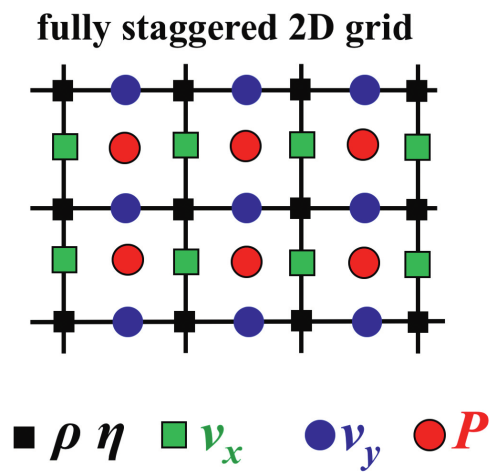
\includegraphics[width=6cm]{images/fdm/gerya_A}\\
{\captionfont Taken from Gerya (2019).}
\end{center}

What follows is mostly borrowed from Taras Gerya's book (second edition). 
However I do not like the notations of the book (or rather they do not match
with the ones of this project) so I have changed them (in particular I use 
the `{\tt n-e-w-s}' system, i.e. north-east-west-south, 
and I prefer $\tau$ to  $\sigma'$ for the deviatoric stress tensor.
Also I feel that it makes more sense to start with a regular mesh 
where all cells have the same size $h_x \times h_y$ (as opposed to the book).
Finally, in the book the $y$-axis points downwards while 'my' $y$-axis 
points upwards.

In what follows we assume that we know the value of the density $\rho$
and viscosity $\eta$ on the (black) nodes of the mesh. We here only focus on the 
Stokes equations (mass and momentum conservation equations) and leave the energy
equation aside.

The justification for the particular approach taken below to 
discretise the equations stems from the concept of conservative 
finite differences explained in Section 7.3 of Gerya's book. 


%\newpage
%...............................................
\subsection{Momentum equation: $x$-component}

Let us zoom-in on a node which carries a $u$ unknown. 
We label it ${\color{violet}u_\otimes}$. Its right ('east')  
neighbour is then ${\color{violet}u_{\tt e}}$,
its left ('west') neighbour is ${\color{violet}u_{\tt w}}$, 
its top ('north') neighbour is ${\color{violet}u_{\tt n}}$ and 
its bottom ('south') neighbour is ${\color{violet}u_{\tt s}}$.
Its nearest pressure nodes are ${\color{teal}p_{\tt e}}$ and 
${\color{teal}p_{\tt w}}$, and the $v$ nodes
that surround it are ${\color{orange}v_{\tt sw}}$, 
${\color{orange}v_{\tt se}}$, ${\color{orange}v_{\tt ne}}$ and 
${\color{orange}v_{\tt nw}}$ as shown here:


\begin{multicols}{2}
\begin{flushright} {\tiny {\color{gray} (tikz\_staggered2D\_u.tex)}} \end{flushright}
%~~~~~~~~~~~~~~~~~~~~~~~~~~~~~~~~~~~~~~~~~~~~~~~~~~~~~~~~~~~~~~~~~~~~~~~~~~~~~~~~~~~~~~~~~~~~~~~~~~

\begin{center}
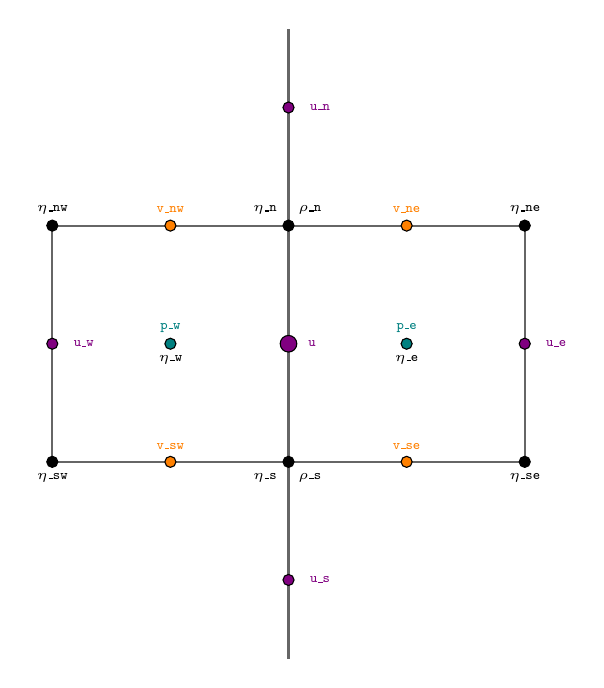
\begin{tikzpicture}
%\draw[fill=gray!23,gray!23](0,0) rectangle (8,9);
%\draw[step=0.5cm,gray,very thin] (0,0) grid (8,9); %background grid

\draw[thick,black!60] (1,3) -- (7,3) -- (7,6) -- (1,6) -- cycle ; 
\draw[thick,black!60] (4,0.5) -- (4,8.5)  ;   

%---------------------------------------------------
\node[] at (2.5,6.2) {\tiny \color{orange} \tt v\_nw};
\node[] at (2.5,3.2) {\tiny \color{orange} \tt v\_sw};
\node[] at (5.5,6.2) {\tiny \color{orange} \tt v\_ne};
\node[] at (5.5,3.2) {\tiny \color{orange} \tt v\_se};
\draw[black,fill=orange] (2.5,6)   circle (2pt);
\draw[black,fill=orange] (2.5,3)   circle (2pt);
\draw[black,fill=orange] (5.5,6)   circle (2pt);
\draw[black,fill=orange] (5.5,3)   circle (2pt);

%--------------------------------------------------
\draw[black,fill=violet] (4,1.5)   circle (2pt);
\draw[black,fill=violet] (4,4.5)   circle (3pt);
\draw[black,fill=violet] (4,7.5)   circle (2pt);
\draw[black,fill=violet] (1,4.5)   circle (2pt);
\draw[black,fill=violet] (7,4.5)   circle (2pt);
\node[] at (4.4,1.5) {\tiny \color{violet} \tt u\_s};
\node[] at (4.3,4.5) {\tiny \color{violet} \tt u};
\node[] at (4.4,7.5) {\tiny \color{violet} \tt u\_n};
\node[] at (1.4,4.5) {\tiny \color{violet} \tt u\_w};
\node[] at (7.4,4.5) {\tiny \color{violet} \tt u\_e};

\draw[black,fill=black] (1,3)   circle (2pt); 
\draw[black,fill=black] (4,3)   circle (2pt); 
\draw[black,fill=black] (7,3)   circle (2pt); 
\draw[black,fill=black] (1,6)   circle (2pt); 
\draw[black,fill=black] (4,6)   circle (2pt); 
\draw[black,fill=black] (7,6)   circle (2pt); 

%------------------------------------------------
\draw[black,fill=teal] (2.5,4.5)   circle (2pt);
\draw[black,fill=teal] (5.5,4.5)   circle (2pt);
\node[] at (2.5,4.7) {\tiny \color{teal} \tt p\_w};
\node[] at (5.5,4.7) {\tiny \color{teal} \tt p\_e};

\node[] at (4.27,2.8) {\tiny \tt $\rho$\_s};
\node[] at (4.27,6.2) {\tiny \tt $\rho$\_n};
\node[] at (2.5,4.3) {\tiny \tt $\eta$\_w};
\node[] at (5.5,4.3) {\tiny \tt $\eta$\_e};
\node[] at (3.7,2.8) {\tiny \tt $\eta$\_s};
\node[] at (3.7,6.2) {\tiny \tt $\eta$\_n};
\node[] at (7,6.2) {\tiny \tt $\eta$\_{ne}};
\node[] at (1,6.2) {\tiny \tt $\eta$\_{nw}};
\node[] at (7,2.8) {\tiny \tt $\eta$\_{se}};
\node[] at (1,2.8) {\tiny \tt $\eta$\_{sw}};
\end{tikzpicture}
\end{center}



\begin{center}
{\captionfont Node layout in {n-e-w-s} notations.}
\end{center}

\columnbreak
\begin{center}
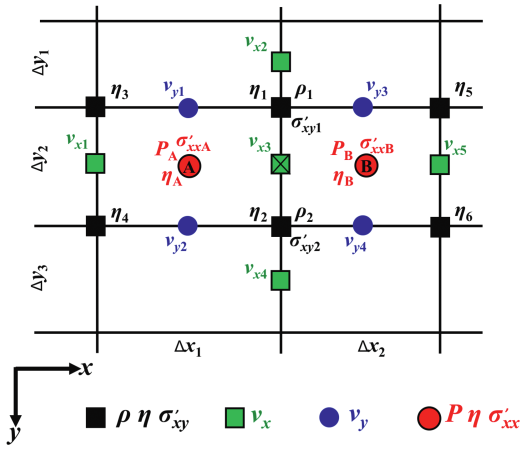
\includegraphics[width=6.5cm]{images/fdm/gerya_B}\\
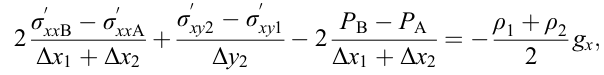
\includegraphics[width=7cm]{images/fdm/gerya_D}\\
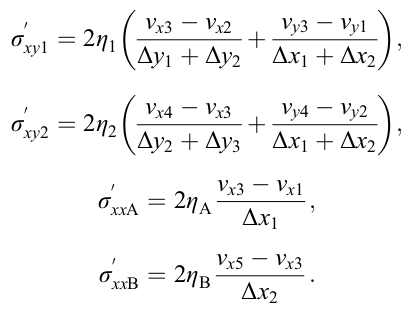
\includegraphics[width=4.5cm]{images/fdm/gerya_F}\\
{\captionfont Taken from Gerya's book}
\end{center}
\end{multicols}

We start from 
\[
\frac{\partial \tau_{xx}}{\partial x}  + 
\frac{\partial \tau_{xy}}{\partial y}  
- \frac{\partial p}{\partial x} + \rho g_x = 0
\]
which we discretise as follows on the purple node in the middle:
\[
\frac{\tau_{xx,{\tt e}}-\tau_{xx,{\tt w}}}{h_x} + \frac{\tau_{xy,{\tt n}}-\tau_{xy,{\tt s}}}{h_y} 
-\frac{{\color{teal}p_{\tt e}}-{\color{teal}p_{\tt w}}}{h_x} 
= -\frac{\rho_{\tt n}+\rho_{\tt s}}{2} g_x
\]
where
\begin{eqnarray}
\tau_{xx,{\tt e}} 
&=& 2 \eta_{\tt e} \dot{\varepsilon}_{xx,{\tt e}} 
= 2\eta_{\tt e} \frac{{\color{violet} u_{\tt e}}-{\color{violet} u_\otimes}}{h_x} \nn \\
\tau_{xx,{\tt w}} 
&=& 2 \eta_{\tt w} \dot{\varepsilon}_{xx,{\tt w}} 
= 2\eta_{\tt w} \frac{{\color{violet} u_\otimes}-{\color{violet} u_{\tt w}}}{h_x} \nn\\
\tau_{xy,{\tt n}} &=& 2 \eta_{\tt n} \dot{\varepsilon}_{xy,{\tt n}} 
= \eta_{\tt n} \left( \frac{{\color{violet} u_{\tt n}}-{\color{violet} u_\otimes}}{h_y} 
+\frac{{\color{orange} v_{\tt ne}}-{\color{orange} v_{\tt nw}}}{h_x} \right) \nn\\
\tau_{xy,{\tt s}} &=& 2 \eta_{\tt s} \dot{\varepsilon}_{xy,{\tt s}} 
= \eta_{\tt s} \left( \frac{{\color{violet} u_\otimes}-{\color{violet} u_{\tt s}}}{h_y} 
+\frac{{\color{orange}v_{\tt se}}-{\color{orange} v_{\tt sw}}}{h_x} \right)  \nn
\end{eqnarray}

We will discuss later in Section~\ref{ss:fdm_stokes_visc} how to arrive at $\eta_{\tt e}$ and $\eta_{\tt w}$.
Inserting the four equations above into the first one, we obtain:
\[
  \frac{1}{h_x} (\tau_{xx,{\tt e}}-\tau_{xx,{\tt w}}) 
+ \frac{1}{h_y} (\tau_{xy,{\tt n}}-\tau_{xy,{\tt s}})
-\frac{1}{h_x} {\color{teal}p_{\tt e}} + \frac{1}{h_x} {\color{teal}p_{\tt w}}
= -\frac{\rho_{\tt n}+\rho_{\tt s}}{2} g_x
\]

{\footnotesize
\[
\frac{1}{h_x} 
\left(  2\eta_{\tt e} \frac{{\color{violet} u_{\tt e}}-{\color{violet} u_\otimes}}{h_x} -  2\eta_{\tt w} \frac{{\color{violet} u_\otimes}-{\color{violet} u_{\tt w}}}{h_x}\right)
+ \frac{1}{h_y} \left[  
\eta_{\tt n} \left( \frac{{\color{violet} u_{\tt n}}-{\color{violet} u_\otimes}}{h_y} +\frac{{\color{orange} v_{\tt ne}}-{\color{orange} v_{\tt nw}}}{h_x} \right)
-
\eta_{\tt s} \left( \frac{{\color{violet} u_\otimes}-{\color{violet} u_{\tt s}}}{h_y} +\frac{{\color{orange} v_{\tt se}}-{\color{orange} v_{\tt sw}}}{h_x} \right) 
\right]
-\frac{1}{h_x} {\color{teal} p_{\tt e}} + \frac{1}{h_x}{\color{teal}p_{\tt w}}
= -\frac{\rho_{\tt n}+\rho_{\tt s}}{2} g_x
\]
}

{\footnotesize
\[
\frac{2\eta_{\tt e}}{h_x}    
\frac{{\color{violet} u_{\tt e}}-{\color{violet} u_\otimes}}{h_x} 
-  \frac{2\eta_{\tt w}}{h_x} \frac{{\color{violet} u_\otimes}-{\color{violet} u_{\tt w}}}{h_x}
+ \frac{\eta_{\tt n}}{h_y}  
 \left( \frac{{\color{violet} u_{\tt n}}-{\color{violet} u_\otimes}}{h_y} +\frac{{\color{orange} v_{\tt ne}}-{\color{orange} v_{\tt nw}}}{h_x} \right)
- \frac{\eta_{\tt s}}{h_y} 
 \left( \frac{{\color{violet} u_\otimes}-{\color{violet} u_{\tt s}}}{h_y} +\frac{{\color{orange} v_{\tt se}}-{\color{orange} v_{\tt sw}}}{h_x} \right) 
-\frac{1}{h_x} {\color{teal}p_{\tt e}} + \frac{1}{h_x} {\color{teal}p_{\tt w}}
= -\frac{\rho_{\tt n}+\rho_{\tt s}}{2} g_x
\]
}


\begin{mdframed}[backgroundcolor=blue!5]
\begin{eqnarray}
\left( \frac{\eta_{\tt n}}{h_y^2} \right) {\color{violet} u_{\tt n}} + 
\left( \frac{2\eta_{\tt e}}{h_x^2} \right) {\color{violet} u_{\tt e}} + 
\left( \frac{2\eta_{\tt w}}{h_x^2} \right) {\color{violet} u_{\tt w}} + 
\left( \frac{\eta_{\tt s}}{h_y^2} \right) {\color{violet} u_{\tt s}} + 
\left( -\frac{2\eta_{\tt e}}{h_x^2} -\frac{2\eta_{\tt w}}{h_x^2}  
-\frac{\eta_{\tt n}}{h_y^2} -\frac{\eta_{\tt s}}{h_y^2}  
\right) {\color{violet} u_\otimes} \nn\\
+
\left( \frac{\eta_{\tt n}}{h_x h_y} \right) {\color{orange} v_{\tt ne}}+ 
\left(-\frac{\eta_{\tt n}}{h_x h_y} \right) {\color{orange} v_{\tt nw}}+ 
\left(-\frac{\eta_{\tt s}}{h_x h_y} \right) {\color{orange} v_{\tt se}}+ 
\left( \frac{\eta_{\tt s}}{h_x h_y} \right) {\color{orange} v_{\tt sw}} 
- \frac{1}{h_x} {\color{teal}p_{\tt e}} + \frac{1}{h_x} {\color{teal}p_{\tt w}} 
&=& -\frac{\rho_{\tt n}+\rho_{\tt s}}{2} g_x \nn\\
\label{eq:fdmstokes1}
\end{eqnarray}
\end{mdframed}




\newpage
%...............................................
\subsection{Momentum equation: $y$-component}

\begin{multicols}{2}
\begin{flushright} {\tiny {\color{gray} (tikz\_staggered2D\_v.tex)}} \end{flushright}
%~~~~~~~~~~~~~~~~~~~~~~~~~~~~~~~~~~~~~~~~~~~~~~~~~~~~~~~~~~~~~~~~~~~~~~~~~~~~~~~~~~~~~~~~~~~~~~~~~~



\begin{center}
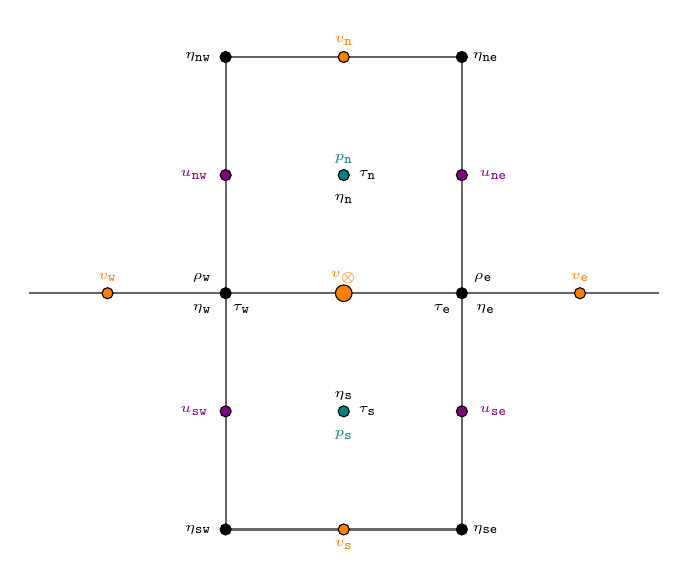
\begin{tikzpicture}
%\draw[fill=gray!23,gray!23](0,0) rectangle (9,8);
%\draw[step=0.5cm,gray,very thin] (0,0) grid (9,8); %background grid
\draw[thick,black!60] (3,1) -- (3,7) -- (6,7) -- (6,1) -- cycle ; 
\draw[thick,black!60] (0.5,4) -- (8.5,4)  ;   
%---------------------------------------------------
\node[] at (4.5,.8) {\tiny \color{orange} $v_{\tt s}$};
\node[] at (4.5,7.2) {\tiny \color{orange} $v_{\tt n}$};
\node[] at (4.5,4.2) {\tiny \color{orange} $v_\otimes$};
\node[] at (1.5,4.2) {\tiny \color{orange} $v_{\tt w}$};
\node[] at (7.5,4.2) {\tiny \color{orange} $v_{\tt e}$};
\draw[black,fill=orange] (4.5,1)   circle (2pt);
\draw[black,fill=orange] (4.5,4)   circle (3pt);
\draw[black,fill=orange] (4.5,7)   circle (2pt);
\draw[black,fill=orange] (1.5,4)   circle (2pt);
\draw[black,fill=orange] (7.5,4)   circle (2pt);
%--------------------------------------------------
\draw[black,fill=violet] (3,2.5)   circle (2pt);
\draw[black,fill=violet] (6,2.5)   circle (2pt);
\draw[black,fill=violet] (3,5.5)   circle (2pt);
\draw[black,fill=violet] (6,5.5)   circle (2pt);
\node[] at (2.6,2.5) {\tiny \color{violet} $u_{\tt sw}$};
\node[] at (6.4,2.5) {\tiny \color{violet} $u_{\tt se}$};
\node[] at (2.6,5.5) {\tiny \color{violet} $u_{\tt nw}$};
\node[] at (6.4,5.5) {\tiny \color{violet} $u_{\tt ne}$};
%-----------------------------------------------
\draw[black,fill=black] (3,1)   circle (2pt); 
\draw[black,fill=black] (3,4)   circle (2pt); 
\draw[black,fill=black] (3,7)   circle (2pt); 
\draw[black,fill=black] (6,1)   circle (2pt); 
\draw[black,fill=black] (6,4)   circle (2pt); 
\draw[black,fill=black] (6,7)   circle (2pt); 
%------------------------------------------------
\draw[black,fill=teal] (4.5,2.5)   circle (2pt);
\draw[black,fill=teal] (4.5,5.5)   circle (2pt);
\node[] at (4.5,2.2) {\tiny \color{teal} $p_{\tt s}$};
\node[] at (4.5,5.7) {\tiny \color{teal} $p_{\tt n}$};
%-----------------------------------------
\node[] at (6.27,4.2) {\tiny $\rho_{\tt e}$};
\node[] at (2.7,4.2) {\tiny $\rho_{\tt w}$};
\node[] at (4.5,5.2) {\tiny $\eta_{\tt n}$};
\node[] at (4.5,2.7) {\tiny $\eta_{\tt s}$};
\node[] at (6.3,1) {\tiny $\eta_{\tt se}$};
\node[] at (2.65,1) {\tiny $\eta_{\tt sw}$};
\node[] at (6.3,7) {\tiny $\eta_{\tt ne}$};
\node[] at (2.65,7) {\tiny $\eta_{\tt nw}$};
\node[] at (6.3,3.8) {\tiny $\eta_{\tt e}$};
\node[] at (2.7,3.8) {\tiny $\eta_{\tt w}$};

\node[] at (3.2,3.8) {\tiny $\tau_{\tt w}$};
\node[] at (5.75,3.8) {\tiny $\tau_{\tt e}$};
\node[] at (4.8,5.5) {\tiny $\tau_{\tt n}$};
\node[] at (4.8,2.5) {\tiny $\tau_{\tt s}$};


\end{tikzpicture}
\end{center}



{\captionfont Node layout in {n-e-w-s} notations.}

\columnbreak

\begin{center}
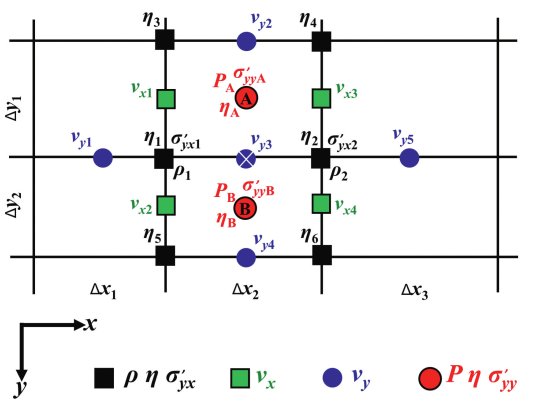
\includegraphics[width=6.5cm]{images/fdm/gerya_C}\\
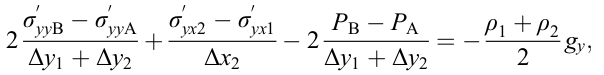
\includegraphics[width=7cm]{images/fdm/gerya_E}\\
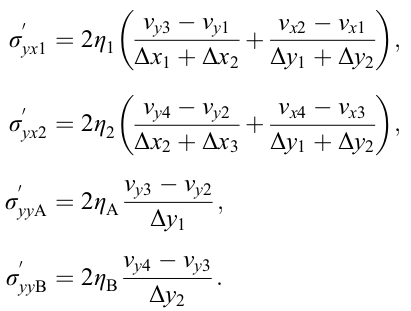
\includegraphics[width=4.5cm]{images/fdm/gerya_G}\\
{\captionfont Taken from Gerya's book}
\end{center}
\end{multicols}


We start from 
\[
\frac{\partial \tau_{xy}}{\partial x}  + 
\frac{\partial \tau_{yy}}{\partial y}  
- \frac{\partial p}{\partial y} + \rho g_y = 0
\]
which we discretise as follows on the ${\color{orange} v_\otimes}$ node in the middle
\[
\frac{\tau_{xy,{\tt e}}-\tau_{xy,{\tt w}}}{h_x} + \frac{\tau_{yy,{\tt n}}-\tau_{yy,{\tt s}}}{h_y} 
-\frac{{\color{teal}p_{\tt n}}-{\color{teal}p_{\tt s}}}{h_y} 
= -\frac{\rho_{\tt e}+\rho_{\tt w}}{2} g_y
\]
where
\begin{eqnarray}
\tau_{xy,{\tt e}} 
&=& 2 \eta_{\tt e} \dot{\varepsilon}_{xy,{\tt e}} 
= \eta_{\tt e} \left( \frac{{\color{violet} u_{\tt ne}}-{\color{violet} u_{\tt se}}}{h_y} 
+\frac{{\color{orange} v_{\tt e}}-{\color{orange} v_\otimes}}{h_x} \right) 
\nn \\
\tau_{xy,{\tt w}} 
&=& 2 \eta_{\tt w} \dot{\varepsilon}_{xy,{\tt w}} 
= \eta_{\tt w} \left( \frac{{\color{violet} u_{\tt nw}}-{\color{violet} u_{\tt sw}}}{h_y} 
+\frac{{\color{orange} v_\otimes} - {\color{orange} v_{\tt w}}}{h_x} \right) 
\nn\\
\tau_{yy,{\tt n}} 
&=& 2 \eta_{\tt n} \dot{\varepsilon}_{yy,{\tt n}} 
= 2\eta_{\tt n} \frac{{\color{orange} v_{\tt n}}-{\color{orange} v_\otimes}}{h_y} 
\nn\\
\tau_{yy,{\tt s}} 
&=& 2 \eta_{\tt s} \dot{\varepsilon}_{yy,{\tt s}} 
= 2\eta_{\tt s} \frac{{\color{orange} v_\otimes} -{\color{orange} v_{\tt s}}}{h_y} 
 \nn
\end{eqnarray}

Again, we will discuss later in Section~\ref{ss:fdm_stokes_visc} how to arrive at 
$\eta_{\tt n}$ and $\eta_{\tt s}$.
Inserting the four equations above into the first one, we obtain:



\[
\frac{1}{h_x} \left(\tau_{xy,{\tt e}}-\tau_{xy,{\tt w}}\right) + 
\frac{1}{h_y} \left(\tau_{yy,{\tt n}}-\tau_{yy,{\tt s}}\right)
-\frac{1}{h_y} {\color{teal}p_{\tt n}} + \frac{1}{h_y} {\color{teal}p_{\tt s}}
= -\frac{\rho_{\tt e}+\rho_{\tt w}}{2} g_y
\]



{\footnotesize
\[
\frac{1}{h_x} \left[
\eta_{\tt e} \left( \frac{{\color{violet} u_{\tt ne}}-{\color{violet} u_{\tt se}}}{h_y} 
+\frac{{\color{orange} v_{\tt e}}-{\color{orange} v_\otimes}}{h_x} \right) 
-
\eta_{\tt w} \left( \frac{{\color{violet} u_{\tt nw}}-{\color{violet} u_{\tt sw}}}{h_y} 
+\frac{{\color{orange} v_\otimes} - {\color{orange} v_{\tt w}}}{h_x} \right) 
\right] 
+
\frac{1}{h_y} \left(
2\eta_{\tt n} \frac{{\color{orange} v_{\tt n}}-{\color{orange} v_\otimes}}{h_y} 
-
2\eta_{\tt s} \frac{{\color{orange} v_\otimes} -{\color{orange} v_{\tt s}}}{h_y}
\right)
-\frac{1}{h_y} {\color{teal}p_{\tt n}} + \frac{1}{h_y} {\color{teal}p_{\tt s}}
= -\frac{\rho_{\tt e}+\rho_{\tt w}}{2} g_y
\]
}





{\footnotesize
\[
\frac{\eta_{\tt e}}{h_x} 
 \left( \frac{{\color{violet} u_{\tt ne}}-{\color{violet} u_{\tt se}}}{h_y} 
+\frac{{\color{orange} v_{\tt e}}-{\color{orange} v_\otimes}}{h_x} \right) 
-
\frac{\eta_{\tt w}}{h_x} \left( \frac{{\color{violet} u_{\tt nw}}-{\color{violet} u_{\tt sw}}}{h_y} 
+\frac{{\color{orange} v_\otimes} - {\color{orange} v_{\tt w}}}{h_x} \right) 
+
\frac{2\eta_{\tt n}}{h_y} 
 \frac{{\color{orange} v_{\tt n}}-{\color{orange} v_\otimes}}{h_y} 
-
\frac{2\eta_{\tt s}}{h_y}   \frac{{\color{orange} v_\otimes} -{\color{orange} v_{\tt s}}}{h_y}
-\frac{1}{h_y} {\color{teal}p_{\tt n}} + \frac{1}{h_y} {\color{teal}p_{\tt s}}
= -\frac{\rho_{\tt e}+\rho_{\tt w}}{2} g_y
\]
}

\begin{mdframed}[backgroundcolor=blue!5]
\begin{eqnarray}
\left( \frac{2\eta_{\tt n}}{h_y^2} \right) {\color{orange} v_{\tt n}} +
\left( \frac{ \eta_{\tt e}}{h_x^2} \right) {\color{orange} v_{\tt e}} +
\left( \frac{ \eta_{\tt w}}{h_x^2} \right) {\color{orange} v_{\tt w}} +
\left( \frac{2\eta_{\tt s}}{h_y^2} \right) {\color{orange} v_{\tt s}} +
\left( 
-\frac{\eta_{\tt e}}{h_x^2} 
-\frac{\eta_{\tt w}}{h_x^2} 
-\frac{2\eta_{\tt n}}{h_y^2} 
-\frac{2\eta_{\tt s}}{h_y^2} 
\right) {\color{orange} v_\otimes} \nn\\
+
\left( \frac{\eta_{\tt e}}{h_x h_y} \right) {\color{violet} u_{\tt ne}} +
\left(-\frac{\eta_{\tt e}}{h_x h_y} \right) {\color{violet} u_{\tt se}} +
\left(-\frac{\eta_{\tt w}}{h_x h_y} \right) {\color{violet} u_{\tt nw}} +
\left( \frac{\eta_{\tt w}}{h_x h_y} \right) {\color{violet} u_{\tt sw}} 
-\frac{1}{h_y} {\color{teal}p_{\tt n}} + \frac{1}{h_y} {\color{teal}p_{\tt s}}
&=& -\frac{\rho_{\tt e}+\rho_{\tt w}}{2} g_y \nn\\
\label{eq:fdmstokes2}
\end{eqnarray}
\end{mdframed}


%----------------------------------
\subsection{Continuity equation}

In two dimensions the continuity equation for an incompressible flow is
\[
\vec\nabla \cdot \vec\upnu 
= 
\frac{\partial u}{\partial x} 
+
\frac{\partial v}{\partial y} 
=0
\]
We can isolate one cell:

\begin{flushright} {\tiny {\color{gray} (tikz\_staggered2D\_divv.tex)}} \end{flushright}
%~~~~~~~~~~~~~~~~~~~~~~~~~~~~~~~~~~~~~~~~~~~~~~~~~~~~~~~~~~~~~~~~~~~~~~~~~~~~~~~~~~~~~~~~~~~~~~~~~~


\begin{center}
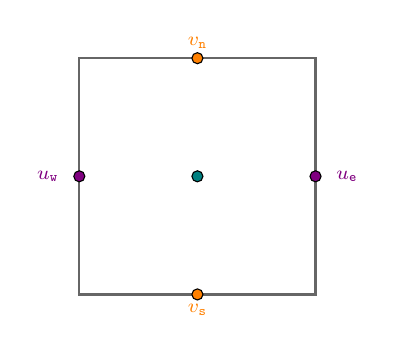
\begin{tikzpicture}
%\draw[fill=gray!23,gray!23](0,0) rectangle (5,5);
%\draw[step=0.5cm,gray,very thin] (0,0) grid (5,5); %background grid
\draw[thick,black!60] (1,1) -- (4,1) -- (4,4) -- (1,4) -- cycle ; 
\draw[black,fill=teal] (2.5,2.5)   circle (2pt);
%---------------------------------------------------
\node[] at (2.5,0.8) {\scriptsize \color{orange} $v_{\tt s}$};
\node[] at (2.5,4.2) {\scriptsize \color{orange} $v_{\tt n}$};
\draw[black,fill=orange] (2.5,1)   circle (2pt);
\draw[black,fill=orange] (2.5,4)   circle (2pt);
%---------------------------------------------------
\node[] at (0.6,2.5) {\scriptsize \color{violet} $u_{\tt w}$};
\node[] at (4.4,2.5) {\scriptsize \color{violet} $u_{\tt e}$};
\draw[black,fill=violet] (1,2.5)   circle (2pt);
\draw[black,fill=violet] (4,2.5)   circle (2pt);
\end{tikzpicture}
\end{center}





and discretise the equation above in its middle.
\begin{mdframed}[backgroundcolor=blue!5]
\begin{equation}
\frac{{\color{violet}u_{\tt e}}-{\color{violet}u_{\tt w}}}{h_x} 
+
\frac{{\color{orange}v_{\tt n}}-{\color{orange}v_{\tt s}}}{h_y} 
=0
\label{eq:fdmstokes3}
\end{equation}
\end{mdframed}



%-------------------------------------------------------------------------
\subsection{Viscosity at the center of cells \label{ss:fdm_stokes_visc} }

Following Gerya, the viscosity in the middle of the cells
can be obtained via averaging (for example arithmetic) of the viscosity values at the corners.

In the case of the $x$-component of the momentum equation:
\[
\eta_{\tt w} = \frac{1}{4}(\eta_{\tt sw}+\eta_{\tt s}+\eta_{\tt n} + \eta_{\tt nw})
\]
\[
\eta_{\tt e} = \frac{1}{4}(\eta_{\tt se}+\eta_{\tt s}+\eta_{\tt n} + \eta_{\tt ne})
\]
In the case of the $y$-component of the momentum equation:
\[
\eta_{\tt n} = \frac{1}{4}(\eta_{\tt w}+\eta_{\tt nw}+\eta_{\tt ne} + \eta_{\tt e})
\]
\[
\eta_{\tt s} = \frac{1}{4}(\eta_{\tt sw}+\eta_{\tt w}+\eta_{\tt e} + \eta_{\tt se})
\]
If harmonic averaging is preferred, then for instance we would have
\[
\eta_{\tt w} = \frac{4}{1/\eta_{\tt sw}+1/\eta_{\tt s}+1/\eta_{\tt n} + 1/\eta_{\tt nw} }
\]


%--------------------------------------------------
\subsection{Boundary conditions}

We start with so-called Dirichlet boundary conditions, i.e. we wish 
to prescribe the value of either velocity components on the boundaries.
For simplicity we will then focus on free slip and no slip boundary conditions.
Free slip b.c. are characterised by a) the normal velocity component on the boundary is zero 
b) the other two components do not change across the boundary (i.e.
zero shear strain rate and shear stresses along the boundary).
No slip b.c. require that all velocity components are zero on the boundary.

Gerya presents in Section 7.4 all the types of boundary conditions but is remarkably elusive 
as to how they should be implemented. Consulting Becker and Kaus, the same conclusion can 
unfortunately be drawn.

Looking at \textcite{hawe65} (1965)
we see that the authors discuss free-slip and no-slip boundary conditions:
\begin{center}
\fbox{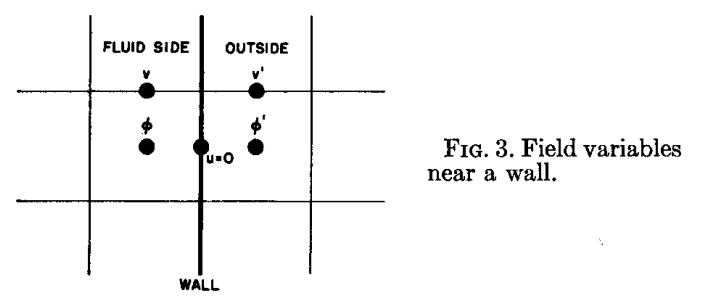
\includegraphics[width=9cm]{images/fdm/hawe65b}}
\end{center}
As mentioned in the paper ``a vertical wall therefore passes through the horizontal-velocity mesh points,
and the velocities at those points vanish at all times for either type of [boundary condition].
A vertical wall does not pass through vertical-velocity mesh points, but the calculation makes use
of the values of $v$ at [virtual] mesh points lying just outside of the wall. For a no-slip wall
the boundary condition is $v'=-v$, while for a free-slip wall it becomes $v'=v$ [on the figure above].''

Let us focus on the bottom of the following mesh:
\begin{center}
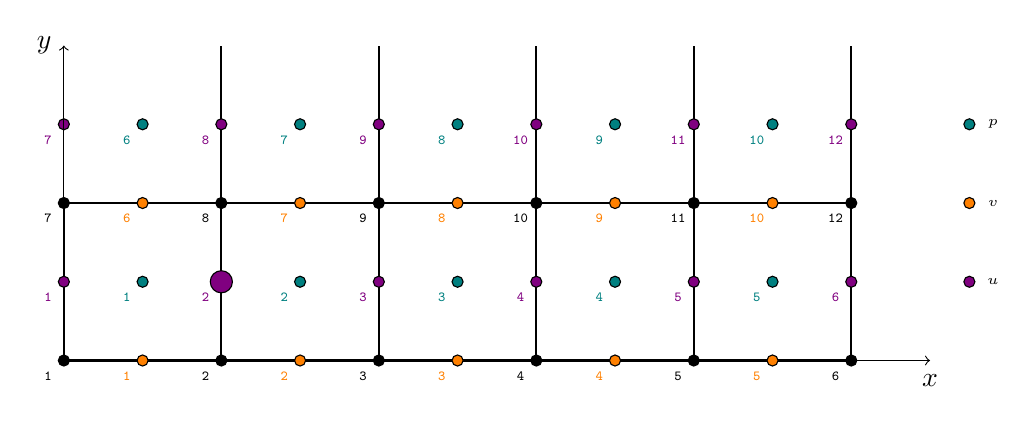
\begin{tikzpicture}
%\draw[fill=gray!23,gray!23](0,0) rectangle (12,10);
%\draw[step=0.5cm,gray,very thin] (0,0) grid (12,10); %background grid

\draw[thick] (0,0) -- (10,0) -- (10,2) -- (0,2) -- cycle ; %1-4
\draw[thick] (0,2) -- (10,2)  ; 
\draw[thick] (2,0) -- (2,4)  ; 
\draw[thick] (4,0) -- (4,4)  ; 
\draw[thick] (6,0) -- (6,4)  ; 
\draw[thick] (8,0) -- (8,4)  ; 
\draw[thick] (10,0) -- (10,4)  ; 
%pressure nodes
\draw[black,fill=teal] (1,1)   circle (2pt); %1
\draw[black,fill=teal] (3,1)   circle (2pt); %1
\draw[black,fill=teal] (5,1)   circle (2pt); %1
\draw[black,fill=teal] (7,1)   circle (2pt); %1
\draw[black,fill=teal] (9,1)   circle (2pt); %1
\draw[black,fill=teal] (1,3)   circle (2pt); %1
\draw[black,fill=teal] (3,3)   circle (2pt); %1
\draw[black,fill=teal] (5,3)   circle (2pt); %1
\draw[black,fill=teal] (7,3)   circle (2pt); %1
\draw[black,fill=teal] (9,3)   circle (2pt); %1
\node[] at (0.8,0.8) {\tiny \color{teal} \tt 1};
\node[] at (2.8,0.8) {\tiny \color{teal} \tt 2};
\node[] at (4.8,0.8) {\tiny \color{teal} \tt 3};
\node[] at (6.8,0.8) {\tiny \color{teal} \tt 4};
\node[] at (8.8,0.8) {\tiny \color{teal} \tt 5};
\node[] at (0.8,2.8) {\tiny \color{teal} \tt 6};
\node[] at (2.8,2.8) {\tiny \color{teal} \tt 7};
\node[] at (4.8,2.8) {\tiny \color{teal} \tt 8};
\node[] at (6.8,2.8) {\tiny \color{teal} \tt 9};
\node[] at (8.8,2.8) {\tiny \color{teal} \tt 10};

% u nodes
\draw[black,fill=violet] (0,1)   circle (2pt); 
\draw[black,fill=violet] (2,1)   circle (4pt); 
\draw[black,fill=violet] (4,1)   circle (2pt); 
\draw[black,fill=violet] (6,1)   circle (2pt); 
\draw[black,fill=violet] (8,1)   circle (2pt); 
\draw[black,fill=violet] (10,1)   circle (2pt);
\draw[black,fill=violet] (0,3)   circle (2pt); 
\draw[black,fill=violet] (2,3)   circle (2pt); 
\draw[black,fill=violet] (4,3)   circle (2pt); 
\draw[black,fill=violet] (6,3)   circle (2pt); 
\draw[black,fill=violet] (8,3)   circle (2pt); 
\draw[black,fill=violet] (10,3)   circle (2pt);


\node[] at (-0.2,0.8) {\tiny \color{violet} \tt 1};
\node[] at (1.8,0.8) {\tiny \color{violet} \tt 2};
\node[] at (3.8,0.8) {\tiny \color{violet} \tt 3};
\node[] at (5.8,0.8) {\tiny \color{violet} \tt 4};
\node[] at (7.8,0.8) {\tiny \color{violet} \tt 5};
\node[] at (9.8,0.8) {\tiny \color{violet} \tt 6};
\node[] at (-0.2,2.8) {\tiny \color{violet} \tt 7};
\node[] at (1.8,2.8) {\tiny \color{violet} \tt 8};
\node[] at (3.8,2.8) {\tiny \color{violet} \tt 9};
\node[] at (5.8,2.8) {\tiny \color{violet} \tt 10};
\node[] at (7.8,2.8) {\tiny \color{violet} \tt 11};
\node[] at (9.8,2.8) {\tiny \color{violet} \tt 12};

% v nodes
\draw[black,fill=orange] (1,0)   circle (2pt); 
\draw[black,fill=orange] (3,0)   circle (2pt); 
\draw[black,fill=orange] (5,0)   circle (2pt); 
\draw[black,fill=orange] (7,0)   circle (2pt); 
\draw[black,fill=orange] (9,0)   circle (2pt); 

\draw[black,fill=orange] (1,2)   circle (2pt); 
\draw[black,fill=orange] (3,2)   circle (2pt); 
\draw[black,fill=orange] (5,2)   circle (2pt); 
\draw[black,fill=orange] (7,2)   circle (2pt); 
\draw[black,fill=orange] (9,2)   circle (2pt); 

\node[] at (0.8,-0.2) {\tiny \color{orange} \tt 1};
\node[] at (2.8,-0.2) {\tiny \color{orange} \tt 2};
\node[] at (4.8,-0.2) {\tiny \color{orange} \tt 3};
\node[] at (6.8,-0.2) {\tiny \color{orange} \tt 4};
\node[] at (8.8,-0.2) {\tiny \color{orange} \tt 5};
\node[] at (0.8,1.8) {\tiny \color{orange} \tt 6};
\node[] at (2.8,1.8) {\tiny \color{orange} \tt 7};
\node[] at (4.8,1.8) {\tiny \color{orange} \tt 8};
\node[] at (6.8,1.8) {\tiny \color{orange} \tt 9};
\node[] at (8.8,1.8) {\tiny \color{orange} \tt 10};
%------------------------------------------------
\draw[black,fill=black] (0,0)   circle (2pt); 
\draw[black,fill=black] (2,0)   circle (2pt); 
\draw[black,fill=black] (4,0)   circle (2pt); 
\draw[black,fill=black] (6,0)   circle (2pt); 
\draw[black,fill=black] (8,0)   circle (2pt); 
\draw[black,fill=black] (10,0)   circle (2pt); 
\draw[black,fill=black] (0,2)   circle (2pt); 
\draw[black,fill=black] (2,2)   circle (2pt); 
\draw[black,fill=black] (4,2)   circle (2pt); 
\draw[black,fill=black] (6,2)   circle (2pt); 
\draw[black,fill=black] (8,2)   circle (2pt); 
\draw[black,fill=black] (10,2)   circle (2pt); 
\node[] at (-0.2,-0.2) {\tiny \tt 1};
\node[] at (1.8,-0.2) {\tiny \tt 2};
\node[] at (3.8,-0.2) {\tiny \tt 3};
\node[] at (5.8,-0.2) {\tiny \tt 4};
\node[] at (7.8,-0.2) {\tiny \tt 5};
\node[] at (9.8,-0.2) {\tiny \tt 6};
\node[] at (-0.2,1.8) {\tiny \tt 7};
\node[] at (1.8,1.8) {\tiny \tt 8};
\node[] at (3.8,1.8) {\tiny \tt 9};
\node[] at (5.8,1.8) {\tiny \tt 10};
\node[] at (7.8,1.8) {\tiny \tt 11};
\node[] at (9.8,1.8) {\tiny \tt 12};
%-------------------------------------------------
\draw[thin,->] (10,0) -- (11,0);  \node[] at (11,-0.25) {$x$};
\draw[thin,->] (0,2) -- (0,4); \node[] at (-0.25,4) {$y$};
%-------------------------------------------------
\draw[black,fill=teal] (11.5,3)   circle (2pt); \node[] at (11.8,3) {\tiny $p$};
\draw[black,fill=orange] (11.5,2)   circle (2pt); \node[] at (11.8,2) {\tiny $v$};
\draw[black,fill=violet] (11.5,1)   circle (2pt); \node[] at (11.8,1) {\tiny $u$};
\end{tikzpicture}
\end{center}



\begin{itemize}
\item \underline{No slip} (at the bottom). We then want $u=v=0$. We can easily zero 
${\color{orange} v_{\tt 1,2,3,4,5}}$ since the corresponding nodes are on the boundary but this is not enough. Let us consider node ${\color{violet}u_{\tt 2}}$ (bigger on the figure above). 
We could zero $u_2$ directly but this would not be correct since the node is not on the boundary.
If we wish to impose $u=0$ exactly on the boundary then its south neighbour ghost value should be set to
-{\color{violet} $u_2$} and used in the established stencils.


\begin{center}
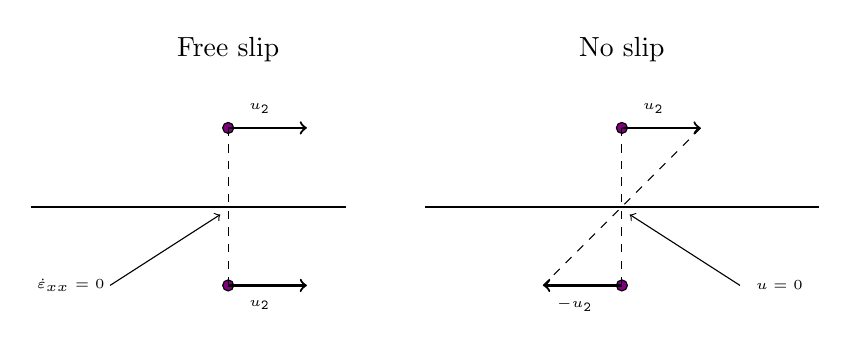
\begin{tikzpicture}
%\draw[fill=gray!23,gray!23](0,0) rectangle (12,6);
%\draw[step=0.5cm,gray,very thin] (0,0) grid (12,6); %background grid
\node[] at (3.5,4) {Free slip};
\node[] at (8.5,4) {No slip};
\draw[thick] (1,2) -- (5,2) ; 
\draw[thick] (6,2) -- (11,2) ; 
\draw[black,fill=violet] (3.5,1)   circle (2pt); 
\draw[black,fill=violet] (3.5,3)   circle (2pt); 
\draw[black,fill=violet] (8.5,1)   circle (2pt); 
\draw[black,fill=violet] (8.5,3)   circle (2pt); 
\draw[dashed] (3.5,1) -- (3.5,3) ; 
\draw[dashed] (8.5,1) -- (8.5,3) ; 
\draw[thin,dashed] (9.5,3) -- (7.5,1) ; 
\draw[thick, ->] (3.5,3)--(4.5,3);
\draw[thick, ->] (3.5,1)--(4.5,1);
\draw[thick, ->] (8.5,3)--(9.5,3);
\draw[thick, ->] (8.5,1)--(7.5,1);
\draw[->] (2,1)--(3.4,1.9);
\node[] at (1.5,1) {\tiny $\dot\varepsilon_{xx}=0$};
\draw[->] (10,1)--(8.6,1.9);
\node[] at (10.5,1) {\tiny $u=0$};

\node[] at (3.9,3.25) {\tiny $u_{\tt 2}$};
\node[] at (3.9,0.75) {\tiny $u_{\tt 2}$};


\node[] at (8.9,3.25) {\tiny $u_{\tt 2}$};
\node[] at (7.9,0.75) {\tiny $-u_{\tt 2}$};

\end{tikzpicture}
\end{center}


\item \underline{Free slip} (at the bottom). Aside from the zero normal velocity 
as above, we also need the tangential velocity gradient to be zero on the boundary, 
which translates into assigning its south neighbour ghost the value +${\color{violet} u_2}$ 
\end{itemize}

We see that in both cases we will need to create ephemeral boundary nodes outside the domain and assign
them specific values based on the boundary condition type. 
This consideration lead Becker \& Kaus to produce this figure in their syllabus:

\begin{center}
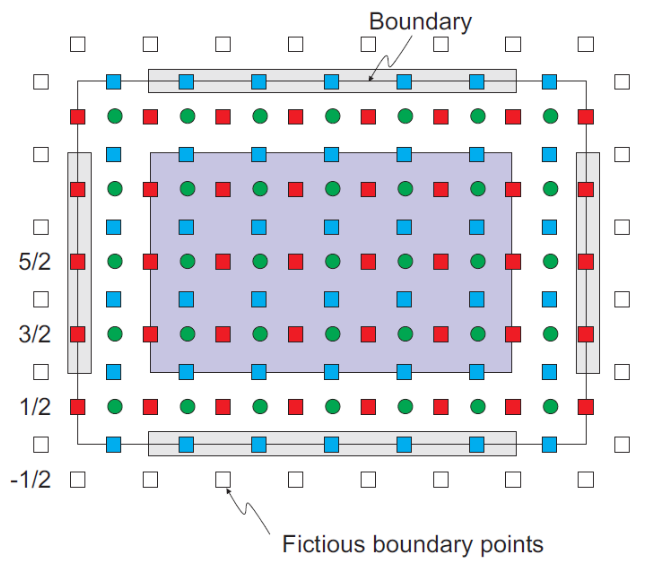
\includegraphics[width=8cm]{images/fdm/bk_A}\\
{\captionfont Taken from \textcite{beka}: Staggered grid definition with the boundary points. 
Within the purple domain, the
finite difference scheme for center points can be applied. At the boundaries, we have to apply a
special finite difference scheme which employs fictitious boundary nodes.}
\end{center}

Let us consider a $4\times 3$ mesh.
We have 12 cells, 15 {\color{violet}$u$}-nodes, 
16 {\color{orange}$v$}-nodes and 12 {\color{teal}$p$}-nodes.
This mesh then counts $N=15+16+12=43$ unknowns\footnote{
Note that the numbering starts at zero, python-style.}.

\begin{flushright} {\tiny {\color{gray} (tikz\_staggered2D\_4x3.tex)}} \end{flushright}
%~~~~~~~~~~~~~~~~~~~~~~~~~~~~~~~~~~~~~~~~~~~~~~~~~~~~~~~~~~~~~~~~~~~~~~~~~~~~~~~~~~~~~~~~~~~~~~~~~~


\begin{center}
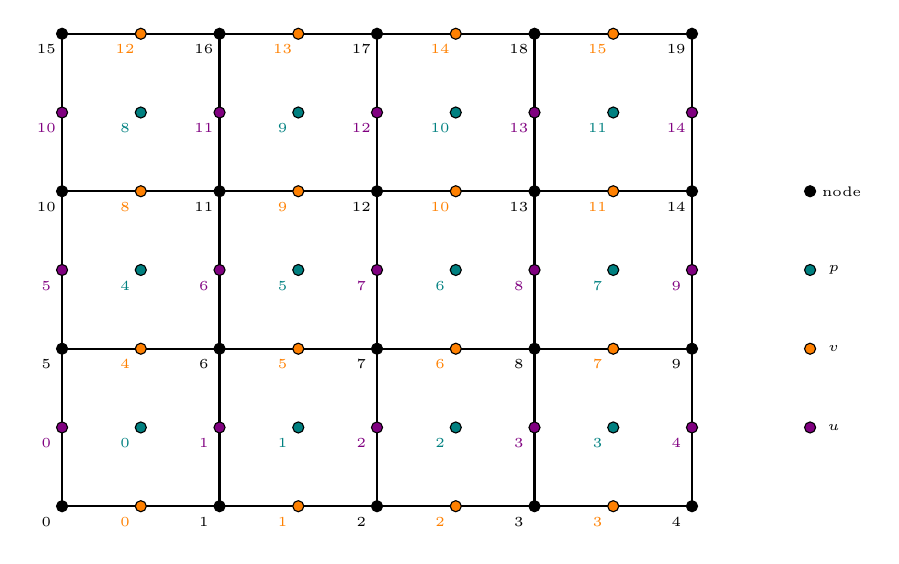
\begin{tikzpicture}
%\draw[fill=gray!23,gray!23](0,0) rectangle (12,10);
%\draw[step=0.5cm,gray,very thin] (0,0) grid (12,10); %background grid

\draw[thick] (0,0) -- (8,0) -- (8,6) -- (0,6) -- cycle ; %1-4
\draw[thick] (0,2) -- (8,2)  ; 
\draw[thick] (0,4) -- (8,4)  ; 
\draw[thick] (2,0) -- (2,6)  ; 
\draw[thick] (4,0) -- (4,6)  ; 
\draw[thick] (6,0) -- (6,6)  ; 

%pressure nodes
\draw[black,fill=teal] (1,1)   circle (2pt); 
\draw[black,fill=teal] (3,1)   circle (2pt); 
\draw[black,fill=teal] (5,1)   circle (2pt); 
\draw[black,fill=teal] (7,1)   circle (2pt); 

\draw[black,fill=teal] (1,3)   circle (2pt); 
\draw[black,fill=teal] (3,3)   circle (2pt); 
\draw[black,fill=teal] (5,3)   circle (2pt); 
\draw[black,fill=teal] (7,3)   circle (2pt); 

\draw[black,fill=teal] (1,5)   circle (2pt); 
\draw[black,fill=teal] (3,5)   circle (2pt); 
\draw[black,fill=teal] (5,5)   circle (2pt); 
\draw[black,fill=teal] (7,5)   circle (2pt); 

\node[] at (0.8,0.8) {\tiny \color{teal} 0};
\node[] at (2.8,0.8) {\tiny \color{teal} 1};
\node[] at (4.8,0.8) {\tiny \color{teal} 2};
\node[] at (6.8,0.8) {\tiny \color{teal} 3};

\node[] at (0.8,2.8) {\tiny \color{teal} 4};
\node[] at (2.8,2.8) {\tiny \color{teal} 5};
\node[] at (4.8,2.8) {\tiny \color{teal} 6};
\node[] at (6.8,2.8) {\tiny \color{teal} 7};

\node[] at (0.8,4.8) {\tiny \color{teal} 8};
\node[] at (2.8,4.8) {\tiny \color{teal} 9};
\node[] at (4.8,4.8) {\tiny \color{teal} 10};
\node[] at (6.8,4.8) {\tiny \color{teal} 11};

% u nodes
\draw[black,fill=violet] (0,1)   circle (2pt); 
\draw[black,fill=violet] (2,1)   circle (2pt); 
\draw[black,fill=violet] (4,1)   circle (2pt); 
\draw[black,fill=violet] (6,1)   circle (2pt); 
\draw[black,fill=violet] (8,1)   circle (2pt); 

\draw[black,fill=violet] (0,3)   circle (2pt); 
\draw[black,fill=violet] (2,3)   circle (2pt); 
\draw[black,fill=violet] (4,3)   circle (2pt); 
\draw[black,fill=violet] (6,3)   circle (2pt);
\draw[black,fill=violet] (8,3)   circle (2pt);

\draw[black,fill=violet] (0,5)   circle (2pt); 
\draw[black,fill=violet] (2,5)   circle (2pt); 
\draw[black,fill=violet] (4,5)   circle (2pt); 
\draw[black,fill=violet] (6,5)   circle (2pt);
\draw[black,fill=violet] (8,5)   circle (2pt);

\node[] at (-0.2,0.8) {\tiny \color{violet} 0};
\node[] at (1.8,0.8)  {\tiny \color{violet} 1};
\node[] at (3.8,0.8)  {\tiny \color{violet} 2};
\node[] at (5.8,0.8)  {\tiny \color{violet} 3};
\node[] at (7.8,0.8)  {\tiny \color{violet} 4};

\node[] at (-0.2,2.8) {\tiny \color{violet} 5};
\node[] at (1.8,2.8)  {\tiny \color{violet} 6};
\node[] at (3.8,2.8)  {\tiny \color{violet} 7};
\node[] at (5.8,2.8)  {\tiny \color{violet} 8};
\node[] at (7.8,2.8)  {\tiny \color{violet} 9};

\node[] at (-0.2,4.8){\tiny \color{violet} 10};
\node[] at (1.8,4.8) {\tiny \color{violet} 11};
\node[] at (3.8,4.8) {\tiny \color{violet} 12};
\node[] at (5.8,4.8) {\tiny \color{violet} 13};
\node[] at (7.8,4.8) {\tiny \color{violet} 14};

% v nodes
\draw[black,fill=orange] (1,0)   circle (2pt); 
\draw[black,fill=orange] (3,0)   circle (2pt); 
\draw[black,fill=orange] (5,0)   circle (2pt); 
\draw[black,fill=orange] (7,0)   circle (2pt); 

\draw[black,fill=orange] (1,2)   circle (2pt); 
\draw[black,fill=orange] (3,2)   circle (2pt); 
\draw[black,fill=orange] (5,2)   circle (2pt); 
\draw[black,fill=orange] (7,2)   circle (2pt); 

\draw[black,fill=orange] (1,4)   circle (2pt); 
\draw[black,fill=orange] (3,4)   circle (2pt); 
\draw[black,fill=orange] (5,4)   circle (2pt); 
\draw[black,fill=orange] (7,4)   circle (2pt); 

\draw[black,fill=orange] (1,6)   circle (2pt); 
\draw[black,fill=orange] (3,6)   circle (2pt); 
\draw[black,fill=orange] (5,6)   circle (2pt); 
\draw[black,fill=orange] (7,6)   circle (2pt); 

\node[] at (0.8,-0.2) {\tiny \color{orange} 0};
\node[] at (2.8,-0.2) {\tiny \color{orange} 1};
\node[] at (4.8,-0.2) {\tiny \color{orange} 2};
\node[] at (6.8,-0.2) {\tiny \color{orange} 3};

\node[] at (0.8,1.8) {\tiny \color{orange} 4};
\node[] at (2.8,1.8) {\tiny \color{orange} 5};
\node[] at (4.8,1.8) {\tiny \color{orange} 6};
\node[] at (6.8,1.8) {\tiny \color{orange} 7};

\node[] at (0.8,3.8) {\tiny \color{orange} 8};
\node[] at (2.8,3.8) {\tiny \color{orange} 9};
\node[] at (4.8,3.8) {\tiny \color{orange} 10};
\node[] at (6.8,3.8) {\tiny \color{orange} 11};

\node[] at (0.8,5.8) {\tiny \color{orange} 12};
\node[] at (2.8,5.8) {\tiny \color{orange} 13};
\node[] at (4.8,5.8) {\tiny \color{orange} 14};
\node[] at (6.8,5.8) {\tiny \color{orange} 15};

%------------------------------------------------

\draw[black,fill=black] (0,0)   circle (2pt); 
\draw[black,fill=black] (2,0)   circle (2pt); 
\draw[black,fill=black] (4,0)   circle (2pt); 
\draw[black,fill=black] (6,0)   circle (2pt); 
\draw[black,fill=black] (8,0)   circle (2pt); 

\draw[black,fill=black] (0,2)   circle (2pt); 
\draw[black,fill=black] (2,2)   circle (2pt); 
\draw[black,fill=black] (4,2)   circle (2pt); 
\draw[black,fill=black] (6,2)   circle (2pt); 
\draw[black,fill=black] (8,2)   circle (2pt); 

\draw[black,fill=black] (0,4)   circle (2pt); 
\draw[black,fill=black] (2,4)   circle (2pt); 
\draw[black,fill=black] (4,4)   circle (2pt); 
\draw[black,fill=black] (6,4)   circle (2pt); 
\draw[black,fill=black] (8,4)   circle (2pt); 

\draw[black,fill=black] (0,6)   circle (2pt); 
\draw[black,fill=black] (2,6)   circle (2pt); 
\draw[black,fill=black] (4,6)   circle (2pt); 
\draw[black,fill=black] (6,6)   circle (2pt); 
\draw[black,fill=black] (8,6)   circle (2pt); 


\node[] at (-0.2,-0.2){\tiny 0};
\node[] at (1.8,-0.2) {\tiny 1};
\node[] at (3.8,-0.2) {\tiny 2};
\node[] at (5.8,-0.2) {\tiny 3};
\node[] at (7.8,-0.2) {\tiny 4};

\node[] at (-0.2,1.8){\tiny 5};
\node[] at (1.8,1.8) {\tiny 6};
\node[] at (3.8,1.8) {\tiny 7};
\node[] at (5.8,1.8) {\tiny 8};
\node[] at (7.8,1.8) {\tiny 9};

\node[] at (-0.2,3.8){\tiny 10};
\node[] at (1.8,3.8) {\tiny 11};
\node[] at (3.8,3.8) {\tiny 12};
\node[] at (5.8,3.8) {\tiny 13};
\node[] at (7.8,3.8) {\tiny 14};

\node[] at (-0.2,5.8){\tiny 15};
\node[] at (1.8,5.8) {\tiny 16};
\node[] at (3.8,5.8) {\tiny 17};
\node[] at (5.8,5.8) {\tiny 18};
\node[] at (7.8,5.8) {\tiny 19};

%-------------------------------------------------

\draw[black,fill=black]  (9.5,4)   circle (2pt); \node[] at (9.9,4) {\tiny node};
\draw[black,fill=teal]   (9.5,3)   circle (2pt); \node[] at (9.8,3) {\tiny $p$};
\draw[black,fill=orange] (9.5,2)   circle (2pt); \node[] at (9.8,2) {\tiny $v$};
\draw[black,fill=violet] (9.5,1)   circle (2pt); \node[] at (9.8,1) {\tiny $u$};

\end{tikzpicture}
\end{center}


Let us assume that we prescribe free slip or no slip on all sides.
Then we must set 
${\color{orange}v_{\tt 0}}={\color{orange}v_{\tt 1}}={\color{orange}v_{\tt 2}}={\color{orange}v_{\tt 3}}={\color{orange}v_{\tt 12}}={\color{orange}v_{\tt 13}}={\color{orange}v_{\tt 14}}={\color{orange}v_{\tt 15}}=0$
and ${\color{violet} u_{\tt 0}}={\color{violet}u_{\tt 4}}={\color{violet}u_{\tt 5}}
={\color{violet}u_{\tt 9}}={\color{violet}u_{\tt 10}} = {\color{violet}u_{\tt 14}}=0$.
This means that we need not discretise the momentum equation on these nodes.

Let us consider node ${\color{violet} u_{7}}$. It has four neighbours so the $x$-component of 
the momentum equation writes there:

\begin{eqnarray}
&&
\left( \frac{\eta_{\tt n}}{h_y^2} \right) {\color{violet} u_{\tt 12}} + 
\left( \frac{2\eta_{\tt e}}{h_x^2} \right) {\color{violet} u_{\tt 8}} + 
\left( \frac{2\eta_{\tt w}}{h_x^2} \right) {\color{violet} u_{\tt 5}} + 
\left( \frac{\eta_{\tt s}}{h_y^2} \right) {\color{violet} u_{\tt 2}} + 
\left( -\frac{2\eta_{\tt e}}{h_x^2} -\frac{2\eta_{\tt w}}{h_x^2}  
-\frac{\eta_{\tt n}}{h_y^2} -\frac{\eta_{\tt s}}{h_y^2}  
\right) {\color{violet} u_7} \nn\\
&&+
\left( \frac{\eta_{\tt n}}{h_x h_y} \right) {\color{orange} v_{\tt 10}}+ 
\left(-\frac{\eta_{\tt n}}{h_x h_y} \right) {\color{orange} v_{\tt 9}}+ 
\left(-\frac{\eta_{\tt s}}{h_x h_y} \right) {\color{orange} v_{\tt 6}}+ 
\left( \frac{\eta_{\tt s}}{h_x h_y} \right) {\color{orange} v_{\tt 5}} 
- \frac{1}{h_x} {\color{teal}p_{\tt 6}} + \frac{1}{h_x} {\color{teal}p_{\tt 5}} = -\frac{\rho_{\tt 12}+\rho_{\tt 7}}{2} g_x 
\nn
\end{eqnarray}





Based on the considerations above pertaining to ghost/virtual nodes
we turn once more to our $4\times 3$ cell mesh where ghost/virtual nodes have been added:

\begin{flushright} {\tiny {\color{gray} (tikz\_staggered2D\_4x3.tex)}} \end{flushright}
%~~~~~~~~~~~~~~~~~~~~~~~~~~~~~~~~~~~~~~~~~~~~~~~~~~~~~~~~~~~~~~~~~~~~~~~~~~~~~~~~~~~~~~~~~~~~~~~~~~


\begin{center}
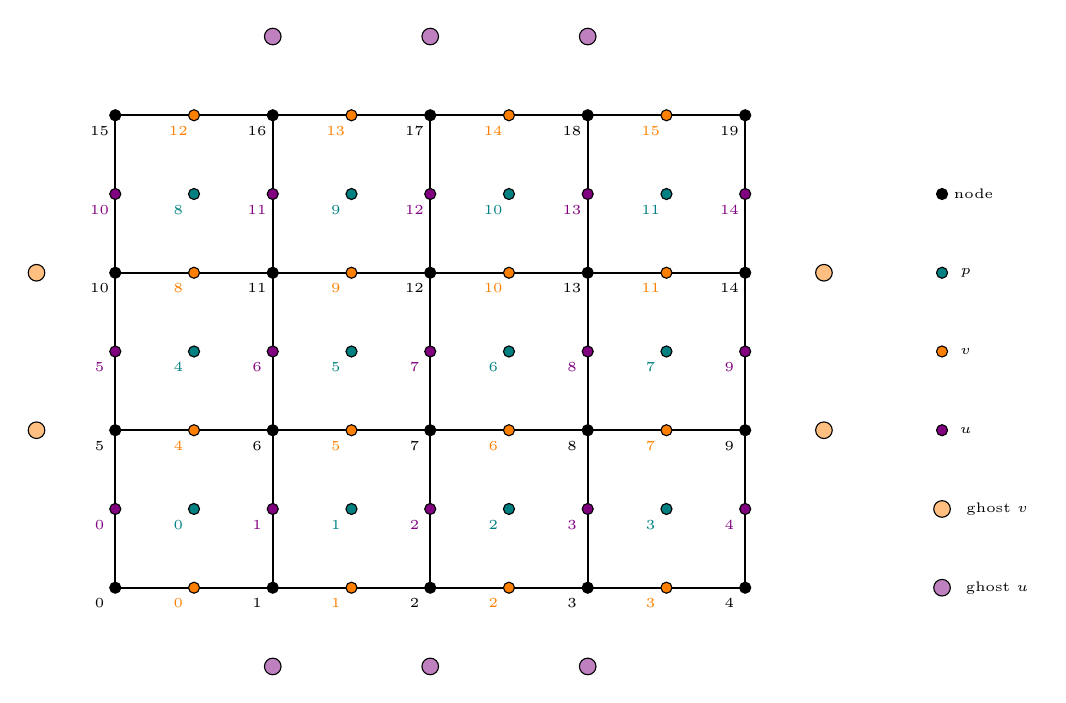
\begin{tikzpicture}
%\draw[fill=gray!23,gray!23](0,0) rectangle (12,10);
%\draw[step=0.5cm,gray,very thin] (0,0) grid (12,10); %background grid

\draw[thick] (0,0) -- (8,0) -- (8,6) -- (0,6) -- cycle ; %1-4
\draw[thick] (0,2) -- (8,2)  ; 
\draw[thick] (0,4) -- (8,4)  ; 
\draw[thick] (2,0) -- (2,6)  ; 
\draw[thick] (4,0) -- (4,6)  ; 
\draw[thick] (6,0) -- (6,6)  ; 

%pressure nodes
\draw[black,fill=teal] (1,1)   circle (2pt); 
\draw[black,fill=teal] (3,1)   circle (2pt); 
\draw[black,fill=teal] (5,1)   circle (2pt); 
\draw[black,fill=teal] (7,1)   circle (2pt); 

\draw[black,fill=teal] (1,3)   circle (2pt); 
\draw[black,fill=teal] (3,3)   circle (2pt); 
\draw[black,fill=teal] (5,3)   circle (2pt); 
\draw[black,fill=teal] (7,3)   circle (2pt); 

\draw[black,fill=teal] (1,5)   circle (2pt); 
\draw[black,fill=teal] (3,5)   circle (2pt); 
\draw[black,fill=teal] (5,5)   circle (2pt); 
\draw[black,fill=teal] (7,5)   circle (2pt); 

\node[] at (0.8,0.8) {\tiny \color{teal} 0};
\node[] at (2.8,0.8) {\tiny \color{teal} 1};
\node[] at (4.8,0.8) {\tiny \color{teal} 2};
\node[] at (6.8,0.8) {\tiny \color{teal} 3};

\node[] at (0.8,2.8) {\tiny \color{teal} 4};
\node[] at (2.8,2.8) {\tiny \color{teal} 5};
\node[] at (4.8,2.8) {\tiny \color{teal} 6};
\node[] at (6.8,2.8) {\tiny \color{teal} 7};

\node[] at (0.8,4.8) {\tiny \color{teal} 8};
\node[] at (2.8,4.8) {\tiny \color{teal} 9};
\node[] at (4.8,4.8) {\tiny \color{teal} 10};
\node[] at (6.8,4.8) {\tiny \color{teal} 11};

% u nodes
\draw[black,fill=violet] (0,1)   circle (2pt); 
\draw[black,fill=violet] (2,1)   circle (2pt); 
\draw[black,fill=violet] (4,1)   circle (2pt); 
\draw[black,fill=violet] (6,1)   circle (2pt); 
\draw[black,fill=violet] (8,1)   circle (2pt); 

\draw[black,fill=violet] (0,3)   circle (2pt); 
\draw[black,fill=violet] (2,3)   circle (2pt); 
\draw[black,fill=violet] (4,3)   circle (2pt); 
\draw[black,fill=violet] (6,3)   circle (2pt);
\draw[black,fill=violet] (8,3)   circle (2pt);

\draw[black,fill=violet] (0,5)   circle (2pt); 
\draw[black,fill=violet] (2,5)   circle (2pt); 
\draw[black,fill=violet] (4,5)   circle (2pt); 
\draw[black,fill=violet] (6,5)   circle (2pt);
\draw[black,fill=violet] (8,5)   circle (2pt);

\node[] at (-0.2,0.8) {\tiny \color{violet} 0};
\node[] at (1.8,0.8)  {\tiny \color{violet} 1};
\node[] at (3.8,0.8)  {\tiny \color{violet} 2};
\node[] at (5.8,0.8)  {\tiny \color{violet} 3};
\node[] at (7.8,0.8)  {\tiny \color{violet} 4};

\node[] at (-0.2,2.8) {\tiny \color{violet} 5};
\node[] at (1.8,2.8)  {\tiny \color{violet} 6};
\node[] at (3.8,2.8)  {\tiny \color{violet} 7};
\node[] at (5.8,2.8)  {\tiny \color{violet} 8};
\node[] at (7.8,2.8)  {\tiny \color{violet} 9};

\node[] at (-0.2,4.8){\tiny \color{violet} 10};
\node[] at (1.8,4.8) {\tiny \color{violet} 11};
\node[] at (3.8,4.8) {\tiny \color{violet} 12};
\node[] at (5.8,4.8) {\tiny \color{violet} 13};
\node[] at (7.8,4.8) {\tiny \color{violet} 14};

% v nodes
\draw[black,fill=orange] (1,0)   circle (2pt); 
\draw[black,fill=orange] (3,0)   circle (2pt); 
\draw[black,fill=orange] (5,0)   circle (2pt); 
\draw[black,fill=orange] (7,0)   circle (2pt); 

\draw[black,fill=orange] (1,2)   circle (2pt); 
\draw[black,fill=orange] (3,2)   circle (2pt); 
\draw[black,fill=orange] (5,2)   circle (2pt); 
\draw[black,fill=orange] (7,2)   circle (2pt); 

\draw[black,fill=orange] (1,4)   circle (2pt); 
\draw[black,fill=orange] (3,4)   circle (2pt); 
\draw[black,fill=orange] (5,4)   circle (2pt); 
\draw[black,fill=orange] (7,4)   circle (2pt); 

\draw[black,fill=orange] (1,6)   circle (2pt); 
\draw[black,fill=orange] (3,6)   circle (2pt); 
\draw[black,fill=orange] (5,6)   circle (2pt); 
\draw[black,fill=orange] (7,6)   circle (2pt); 

\node[] at (0.8,-0.2) {\tiny \color{orange} 0};
\node[] at (2.8,-0.2) {\tiny \color{orange} 1};
\node[] at (4.8,-0.2) {\tiny \color{orange} 2};
\node[] at (6.8,-0.2) {\tiny \color{orange} 3};

\node[] at (0.8,1.8) {\tiny \color{orange} 4};
\node[] at (2.8,1.8) {\tiny \color{orange} 5};
\node[] at (4.8,1.8) {\tiny \color{orange} 6};
\node[] at (6.8,1.8) {\tiny \color{orange} 7};

\node[] at (0.8,3.8) {\tiny \color{orange} 8};
\node[] at (2.8,3.8) {\tiny \color{orange} 9};
\node[] at (4.8,3.8) {\tiny \color{orange} 10};
\node[] at (6.8,3.8) {\tiny \color{orange} 11};

\node[] at (0.8,5.8) {\tiny \color{orange} 12};
\node[] at (2.8,5.8) {\tiny \color{orange} 13};
\node[] at (4.8,5.8) {\tiny \color{orange} 14};
\node[] at (6.8,5.8) {\tiny \color{orange} 15};

%------------------------------------------------

\draw[black,fill=black] (0,0)   circle (2pt); 
\draw[black,fill=black] (2,0)   circle (2pt); 
\draw[black,fill=black] (4,0)   circle (2pt); 
\draw[black,fill=black] (6,0)   circle (2pt); 
\draw[black,fill=black] (8,0)   circle (2pt); 

\draw[black,fill=black] (0,2)   circle (2pt); 
\draw[black,fill=black] (2,2)   circle (2pt); 
\draw[black,fill=black] (4,2)   circle (2pt); 
\draw[black,fill=black] (6,2)   circle (2pt); 
\draw[black,fill=black] (8,2)   circle (2pt); 

\draw[black,fill=black] (0,4)   circle (2pt); 
\draw[black,fill=black] (2,4)   circle (2pt); 
\draw[black,fill=black] (4,4)   circle (2pt); 
\draw[black,fill=black] (6,4)   circle (2pt); 
\draw[black,fill=black] (8,4)   circle (2pt); 

\draw[black,fill=black] (0,6)   circle (2pt); 
\draw[black,fill=black] (2,6)   circle (2pt); 
\draw[black,fill=black] (4,6)   circle (2pt); 
\draw[black,fill=black] (6,6)   circle (2pt); 
\draw[black,fill=black] (8,6)   circle (2pt); 


\node[] at (-0.2,-0.2){\tiny 0};
\node[] at (1.8,-0.2) {\tiny 1};
\node[] at (3.8,-0.2) {\tiny 2};
\node[] at (5.8,-0.2) {\tiny 3};
\node[] at (7.8,-0.2) {\tiny 4};

\node[] at (-0.2,1.8){\tiny 5};
\node[] at (1.8,1.8) {\tiny 6};
\node[] at (3.8,1.8) {\tiny 7};
\node[] at (5.8,1.8) {\tiny 8};
\node[] at (7.8,1.8) {\tiny 9};

\node[] at (-0.2,3.8){\tiny 10};
\node[] at (1.8,3.8) {\tiny 11};
\node[] at (3.8,3.8) {\tiny 12};
\node[] at (5.8,3.8) {\tiny 13};
\node[] at (7.8,3.8) {\tiny 14};

\node[] at (-0.2,5.8){\tiny 15};
\node[] at (1.8,5.8) {\tiny 16};
\node[] at (3.8,5.8) {\tiny 17};
\node[] at (5.8,5.8) {\tiny 18};
\node[] at (7.8,5.8) {\tiny 19};

%-------------------------------------------------

\draw[black,fill=black]  (10.5,5)   circle (2pt); \node[] at (10.9,5) {\tiny node};
\draw[black,fill=teal]   (10.5,4)   circle (2pt); \node[] at (10.8,4) {\tiny $p$};
\draw[black,fill=orange] (10.5,3)   circle (2pt); \node[] at (10.8,3) {\tiny $v$};
\draw[black,fill=violet] (10.5,2)   circle (2pt); \node[] at (10.8,2) {\tiny $u$};

\draw[black,fill=orange!50] (10.5,1)  circle (3pt); \node[] at (11.2,1) {\tiny ghost $v$};
\draw[black,fill=violet!50] (10.5,0)  circle (3pt); \node[] at (11.2,0) {\tiny ghost $u$};

%boundary u nodes
\draw[black,fill=violet!50] (2,-1)   circle (3pt); 
\draw[black,fill=violet!50] (4,-1)   circle (3pt); 
\draw[black,fill=violet!50] (6,-1)   circle (3pt); 
\draw[black,fill=violet!50] (2,7)   circle (3pt); 
\draw[black,fill=violet!50] (4,7)   circle (3pt); 
\draw[black,fill=violet!50] (6,7)   circle (3pt); 

%boundary u nodes
\draw[black,fill=orange!50] (-1,2)   circle (3pt); 
\draw[black,fill=orange!50] (-1,4)   circle (3pt); 
\draw[black,fill=orange!50] (9,2)   circle (3pt); 
\draw[black,fill=orange!50] (9,4)   circle (3pt); 





\end{tikzpicture}
\end{center}



\begin{itemize}
\item ${\color{violet} u_{\tt 0,5,10}}$: situated on left boundary. Free slip and no slip require ${\color{violet} u}=0$. No need for a ghost node.
\item ${\color{violet} u_{\tt 4,9,14}}$: situated on right boundary. Free slip and no slip require ${\color{violet} u}=0$. No need for a ghost node.
\item ${\color{violet} u_{\tt 1,2,3}}$: north, east, west neighbours are present, but south is missing so south ghost nodes are needed.

Let us write the stencil for these nodes:
\begin{eqnarray}
\left( \frac{\eta_{\tt n}}{h_y^2} \right) {\color{violet} u_{\tt n}} + 
\left( \frac{2\eta_{\tt e}}{h_x^2} \right) {\color{violet} u_{\tt e}} + 
\left( \frac{2\eta_{\tt w}}{h_x^2} \right) {\color{violet} u_{\tt w}} + 
\boxed{\left( \frac{\eta_{\tt s}}{h_y^2} \right) {\color{violet} u_{\tt s}}} + 
\left( -\frac{2\eta_{\tt e}}{h_x^2} -\frac{2\eta_{\tt w}}{h_x^2}  
-\frac{\eta_{\tt n}}{h_y^2} -\frac{\eta_{\tt s}}{h_y^2}  
\right) {\color{violet} u_\otimes} \nn\\
+
\left( \frac{\eta_{\tt n}}{h_x h_y} \right) {\color{orange} v_{\tt ne}}+ 
\left(-\frac{\eta_{\tt n}}{h_x h_y} \right) {\color{orange} v_{\tt nw}}+ 
\left(-\frac{\eta_{\tt s}}{h_x h_y} \right) {\color{orange} v_{\tt se}}+ 
\left( \frac{\eta_{\tt s}}{h_x h_y} \right) {\color{orange} v_{\tt sw}} 
- \frac{1}{h_x} {\color{teal}p_{\tt e}} + \frac{1}{h_x} {\color{teal}p_{\tt w}} 
&=& -\frac{\rho_{\tt n}+\rho_{\tt s}}{2} g_x \nn
\end{eqnarray}
As we have seen earlier there is obviously a problem as ${\color{violet} u_{\tt s}}$ (the boxed term)
is not defined.
If we wish to prescribe free slip, we have seen that we must set 
${\color{violet} u_{\tt s}}={\color{violet} u_\otimes}$.
If we wish to prescribe no slip, we have seen that we must set 
${\color{violet} u_{\tt s}}=-{\color{violet} u_\otimes}$.
The stencil then becomes:
\begin{eqnarray}
\left( \frac{\eta_{\tt n}}{h_y^2} \right) {\color{violet} u_{\tt n}} + 
\left( \frac{2\eta_{\tt e}}{h_x^2} \right) {\color{violet} u_{\tt e}} + 
\left( \frac{2\eta_{\tt w}}{h_x^2} \right) {\color{violet} u_{\tt w}} + 
\left( -\frac{2\eta_{\tt e}}{h_x^2} -\frac{2\eta_{\tt w}}{h_x^2}  
-\frac{\eta_{\tt n}}{h_y^2} -(1-\delta_{bc})\frac{\eta_{\tt s}}{h_y^2}
\right) {\color{violet} u_\otimes} \nn\\
+
\left( \frac{\eta_{\tt n}}{h_x h_y} \right) {\color{orange} v_{\tt ne}}+ 
\left(-\frac{\eta_{\tt n}}{h_x h_y} \right) {\color{orange} v_{\tt nw}}+ 
\left(-\frac{\eta_{\tt s}}{h_x h_y} \right) {\color{orange} v_{\tt se}}+ 
\left( \frac{\eta_{\tt s}}{h_x h_y} \right) {\color{orange} v_{\tt sw}} 
- \frac{1}{h_x} {\color{teal}p_{\tt e}} + \frac{1}{h_x} {\color{teal}p_{\tt w}} 
&=& -\frac{\rho_{\tt n}+\rho_{\tt s}}{2} g_x \nn
\end{eqnarray}
where $\delta_{bc}=1$ (free slip) or -1 (no slip).



\item ${\color{violet} u_{\tt 11,12,13}}$: south, east, west neighbours are present, but north is missing so north ghost nodes are needed.

Let us write the stencil for these nodes:
\begin{eqnarray}
\boxed{\left( \frac{\eta_{\tt n}}{h_y^2} \right) {\color{violet} u_{\tt n}}} + 
\left( \frac{2\eta_{\tt e}}{h_x^2} \right) {\color{violet} u_{\tt e}} + 
\left( \frac{2\eta_{\tt w}}{h_x^2} \right) {\color{violet} u_{\tt w}} + 
\left( \frac{\eta_{\tt s}}{h_y^2} \right) {\color{violet} u_{\tt s}} + 
\left( -\frac{2\eta_{\tt e}}{h_x^2} -\frac{2\eta_{\tt w}}{h_x^2}  
-\frac{\eta_{\tt n}}{h_y^2} -\frac{\eta_{\tt s}}{h_y^2}  
\right) {\color{violet} u_\otimes} \nn\\
+
\left( \frac{\eta_{\tt n}}{h_x h_y} \right) {\color{orange} v_{\tt ne}}+ 
\left(-\frac{\eta_{\tt n}}{h_x h_y} \right) {\color{orange} v_{\tt nw}}+ 
\left(-\frac{\eta_{\tt s}}{h_x h_y} \right) {\color{orange} v_{\tt se}}+ 
\left( \frac{\eta_{\tt s}}{h_x h_y} \right) {\color{orange} v_{\tt sw}} 
- \frac{1}{h_x} {\color{teal}p_{\tt e}} + \frac{1}{h_x} {\color{teal}p_{\tt w}} 
&=& -\frac{\rho_{\tt n}+\rho_{\tt s}}{2} g_x \nn
\end{eqnarray}
Here again there is obviously a problem as ${\color{violet} u_{\tt n}}$ is not defined (boxed term).
Using the same $\delta_{bc}$ parameter the stencil then becomes:
\begin{eqnarray}
\left( \frac{2\eta_{\tt e}}{h_x^2} \right) {\color{violet} u_{\tt e}} + 
\left( \frac{2\eta_{\tt w}}{h_x^2} \right) {\color{violet} u_{\tt w}} + 
\left( \frac{\eta_{\tt s}}{h_y^2} \right) {\color{violet} u_{\tt s}} + 
\left( -\frac{2\eta_{\tt e}}{h_x^2} -\frac{2\eta_{\tt w}}{h_x^2}  
-(1-\delta_{bc})\frac{\eta_{\tt n}}{h_y^2} -\frac{\eta_{\tt s}}{h_y^2}  
\right) {\color{violet} u_\otimes} \nn\\
+
\left( \frac{\eta_{\tt n}}{h_x h_y} \right) {\color{orange} v_{\tt ne}}+ 
\left(-\frac{\eta_{\tt n}}{h_x h_y} \right) {\color{orange} v_{\tt nw}}+ 
\left(-\frac{\eta_{\tt s}}{h_x h_y} \right) {\color{orange} v_{\tt se}}+ 
\left( \frac{\eta_{\tt s}}{h_x h_y} \right) {\color{orange} v_{\tt sw}} 
- \frac{1}{h_x} {\color{teal}p_{\tt e}} + \frac{1}{h_x} {\color{teal}p_{\tt w}} 
&=& -\frac{\rho_{\tt n}+\rho_{\tt s}}{2} g_x \nn
\end{eqnarray}



\item ${\color{violet} u_{\tt 6,7,8}}$: standard stencil applies as 
these nodes have four `real' neighbours.
\item ${\color{orange} v_{\tt 0,1,2,3}}$: situated on bottom boundary. Free slip and no slip require ${\color{orange} v}=0$. No need for a ghost node.
\item ${\color{orange} v_{\tt 12,13,14,15}}$: situated on top boundary. Free slip and no slip require ${\color{orange} v}=0$. No need for a ghost node.

\item ${\color{orange} v_{\tt 4,8}}$: north, east, south neighbours are present, but west is missing so west ghost nodes are needed.
\begin{eqnarray}
\left( \frac{2\eta_{\tt n}}{h_y^2} \right) {\color{orange} v_{\tt n}} +
\left( \frac{ \eta_{\tt e}}{h_x^2} \right) {\color{orange} v_{\tt e}} +
\boxed{\left( \frac{ \eta_{\tt w}}{h_x^2} \right) {\color{orange} v_{\tt w}}} +
\left( \frac{2\eta_{\tt s}}{h_y^2} \right) {\color{orange} v_{\tt s}} +
\left( 
-\frac{\eta_{\tt e}}{h_x^2} 
-\frac{\eta_{\tt w}}{h_x^2} 
-\frac{2\eta_{\tt n}}{h_y^2} 
-\frac{2\eta_{\tt s}}{h_y^2} 
\right) {\color{orange} v_\otimes} \nn\\
+
\left( \frac{\eta_{\tt e}}{h_x h_y} \right) {\color{violet} u_{\tt ne}} +
\left(-\frac{\eta_{\tt e}}{h_x h_y} \right) {\color{violet} u_{\tt se}} +
\left(-\frac{\eta_{\tt w}}{h_x h_y} \right) {\color{violet} u_{\tt nw}} +
\left( \frac{\eta_{\tt w}}{h_x h_y} \right) {\color{violet} u_{\tt sw}} 
-\frac{1}{h_y} {\color{teal}p_{\tt n}} + \frac{1}{h_y} {\color{teal}p_{\tt s}}
&=& -\frac{\rho_{\tt e}+\rho_{\tt w}}{2} g_y \nn
\end{eqnarray}
leads to
\begin{eqnarray}
\left( \frac{2\eta_{\tt n}}{h_y^2} \right) {\color{orange} v_{\tt n}} +
\left( \frac{ \eta_{\tt e}}{h_x^2} \right) {\color{orange} v_{\tt e}} +
\left( \frac{2\eta_{\tt s}}{h_y^2} \right) {\color{orange} v_{\tt s}} +
\left( 
-\frac{\eta_{\tt e}}{h_x^2} 
-(1-\delta_{bc})\frac{\eta_{\tt w}}{h_x^2} 
-\frac{2\eta_{\tt n}}{h_y^2} 
-\frac{2\eta_{\tt s}}{h_y^2} 
\right) {\color{orange} v_\otimes} \nn\\
+
\left( \frac{\eta_{\tt e}}{h_x h_y} \right) {\color{violet} u_{\tt ne}} +
\left(-\frac{\eta_{\tt e}}{h_x h_y} \right) {\color{violet} u_{\tt se}} +
\left(-\frac{\eta_{\tt w}}{h_x h_y} \right) {\color{violet} u_{\tt nw}} +
\left( \frac{\eta_{\tt w}}{h_x h_y} \right) {\color{violet} u_{\tt sw}} 
-\frac{1}{h_y} {\color{teal}p_{\tt n}} + \frac{1}{h_y} {\color{teal}p_{\tt s}}
&=& -\frac{\rho_{\tt e}+\rho_{\tt w}}{2} g_y \nn
\end{eqnarray}



\item ${\color{orange} v_{\tt 7,11}}$: south,  west, north neighbours are present, but east is missing so east ghost nodes are needed.
\begin{eqnarray}
\left( \frac{2\eta_{\tt n}}{h_y^2} \right) {\color{orange} v_{\tt n}} +
\boxed{\left( \frac{ \eta_{\tt e}}{h_x^2} \right) {\color{orange} v_{\tt e}}} +
\left( \frac{ \eta_{\tt w}}{h_x^2} \right) {\color{orange} v_{\tt w}} +
\left( \frac{2\eta_{\tt s}}{h_y^2} \right) {\color{orange} v_{\tt s}} +
\left( 
-\frac{\eta_{\tt e}}{h_x^2} 
-\frac{\eta_{\tt w}}{h_x^2} 
-\frac{2\eta_{\tt n}}{h_y^2} 
-\frac{2\eta_{\tt s}}{h_y^2} 
\right) {\color{orange} v_\otimes} \nn\\
+
\left( \frac{\eta_{\tt e}}{h_x h_y} \right) {\color{violet} u_{\tt ne}} +
\left(-\frac{\eta_{\tt e}}{h_x h_y} \right) {\color{violet} u_{\tt se}} +
\left(-\frac{\eta_{\tt w}}{h_x h_y} \right) {\color{violet} u_{\tt nw}} +
\left( \frac{\eta_{\tt w}}{h_x h_y} \right) {\color{violet} u_{\tt sw}} 
-\frac{1}{h_y} {\color{teal}p_{\tt n}} + \frac{1}{h_y} {\color{teal}p_{\tt s}}
&=& -\frac{\rho_{\tt e}+\rho_{\tt w}}{2} g_y \nn
\end{eqnarray}
leads to
\begin{eqnarray}
\left( \frac{2\eta_{\tt n}}{h_y^2} \right) {\color{orange} v_{\tt n}} +
\left( \frac{ \eta_{\tt w}}{h_x^2} \right) {\color{orange} v_{\tt w}} +
\left( \frac{2\eta_{\tt s}}{h_y^2} \right) {\color{orange} v_{\tt s}} +
\left( 
-(1-\delta_{bc})\frac{\eta_{\tt e}}{h_x^2} 
-\frac{\eta_{\tt w}}{h_x^2} 
-\frac{2\eta_{\tt n}}{h_y^2} 
-\frac{2\eta_{\tt s}}{h_y^2} 
\right) {\color{orange} v_\otimes} \nn\\
+
\left( \frac{\eta_{\tt e}}{h_x h_y} \right) {\color{violet} u_{\tt ne}} +
\left(-\frac{\eta_{\tt e}}{h_x h_y} \right) {\color{violet} u_{\tt se}} +
\left(-\frac{\eta_{\tt w}}{h_x h_y} \right) {\color{violet} u_{\tt nw}} +
\left( \frac{\eta_{\tt w}}{h_x h_y} \right) {\color{violet} u_{\tt sw}} 
-\frac{1}{h_y} {\color{teal}p_{\tt n}} + \frac{1}{h_y} {\color{teal}p_{\tt s}}
&=& -\frac{\rho_{\tt e}+\rho_{\tt w}}{2} g_y \nn
\end{eqnarray}


\item ${\color{orange} v_{\tt 5,6,9,10}}$: standard stencil applies as these nodes have four 'real' neighbours.
\item pressure nodes are situated inside each cell and are unaffected by the type of boundary conditions
since the stencil of the continuity equation is always complete (no need for ghost nodes).
\end{itemize}

Note that if free slip or no slip boundary conditions are prescribed on all four boundaries the 
pressure solution is only known up to a constant. Often this pressure nullspace is removed 
from the solution since most solvers will happily solve the linear system even though it is not 
strictly definite. Gerya advocates to set a zero boundary condition on a node (and then re-normalise the 
pressure).

In practice ghost nodes are never created or used. They are useful in order to 
establish the corrected stencils but are entirely absent from the coding.

%---------------------------------------------------
\subsection{Generating the linear system}

Let us now create the vector $\vec{X}$ that is $N=N_u+N_v+N_p=43$ long 
(still considering 
the $4\times 3$ cell mesh presented above):
\[
\vec{X}^T=(\vec{\cal U}, \vec{\cal V}, \vec{\cal P} )=(
u_{\tt \color{violet} 0},u_{\tt \color{violet} 1}, \dots , u_{\tt \color{violet} 14},
v_{\tt \color{orange} 0},v_{\tt \color{orange} 1}, \dots , v_{\tt \color{orange} 15},
p_{\tt \color{teal} 0},p_{\tt \color{teal} 1}, \dots, p_{\tt \color{teal} 11})
\]
We have 14 boundary conditions and 29 stencil equations that establish relationships between 
unknowns  (see previous section) which we can write altogether as a linear system.

The boundary condition $u_{\color{violet} \tt 0}=0$ can be written 
\[
(1,0,0,0,...,0) \cdot \vec{X} = (0,....)^T
\]
so that the lhs horizontal vector becomes the first line of the matrix and we
must write zero in the first element of the rhs vector. 

Likewise the boundary condition $u_{\color{violet} \tt 4}=0$ can be written
\[
(0,0,0,0,1,...,0) \cdot \vec{X} = (.,.,.,.,0,....)^T
\]
and the lhs horizontal vector becomes the 5th line of the matrix and we
must write zero in the 5th element of the rhs vector. 

We repeat this procedure for all $u$ boundary conditions, which allows us to fill 
the 1st, 5th, 6th, 10th, 11th and 14th line of the matrix.

Likewise the boundary conditions on $v$ will yield similar lines in the matrix, 
only the corresponding lines are below the 15 first ones corresponding to $u$.

Considering node ${\color{violet} u_7}$, the stencil equation \eqref{eq:fdmstokes1} then becomes:



\begin{eqnarray}
\left( \frac{\eta_{\tt n}}{h_y^2} \right) {\color{violet} u_{\tt 12}} + 
\left( \frac{2\eta_{\tt e}}{h_x^2} \right) {\color{violet} u_{\tt 8}} + 
\left( \frac{2\eta_{\tt w}}{h_x^2} \right) {\color{violet} u_{\tt 6}} + 
\left( \frac{\eta_{\tt s}}{h_y^2} \right) {\color{violet} u_{\tt 2}} + 
\left( -\frac{2\eta_{\tt e}}{h_x^2} -\frac{2\eta_{\tt w}}{h_x^2}  
-\frac{\eta_{\tt n}}{h_y^2} -\frac{\eta_{\tt s}}{h_y^2}  
\right) {\color{violet} u_7} \nn\\
+
\left( \frac{\eta_{\tt n}}{h_x h_y} \right) {\color{orange} v_{\tt 10}}+ 
\left(-\frac{\eta_{\tt n}}{h_x h_y} \right) {\color{orange} v_{\tt 9}}+ 
\left(-\frac{\eta_{\tt s}}{h_x h_y} \right) {\color{orange} v_{\tt 6}}+ 
\left( \frac{\eta_{\tt s}}{h_x h_y} \right) {\color{orange} v_{\tt 5}} 
- \frac{1}{h_x} {\color{teal}p_{\tt 6}} + \frac{1}{h_x} {\color{teal}p_{\tt 5}} 
&=& -\frac{\rho_{\tt 12}+\rho_{\tt 7}}{2} g_x \nn
\end{eqnarray}
which will correspond to the 7th line in the matrix. The coefficients inside the 
parentheses will be input in the column corresponding to the unknowns they front. 



Because of how the $\vec{X}$ vector is built (first ${\color{violet} u}$, 
then ${\color{orange}v}$ then ${\color{teal} p}$ unknowns)
the resulting linear system takes the following form:
\begin{equation}
\left(
\begin{array}{ccc}
\K_{xx} & \K_{xy} & \G_x \\
\K_{yx} & \K_{yy} & \G_y \\
\Q_x & \Q_y & 0
\end{array}
\right)
\cdot
\vec{X}
=\vec{b}
\label{eq:fdmstokes6}
\end{equation}











%--------------------------------------------------
\subsection{A remark about scaling of terms}

The coefficients before the velocity components are all of the form 
$\eta/h^2$ while those in front of the pressure terms are of the form 
$1/h$. 

In geodynamics typical velocities are of the order of a cm/year, or about 
$10^{-10}$ m/s
while typical pressures are on the order of 1 GPa.
For a viscosity of about $10^{21}$Pa, and a mesh size of about 1km, 
we have:
\[
\frac{\eta}{h^2} v \sim \frac{10^{21}}{1000^2} 10^{-10} \sim 10^6
\]
while
\[
\frac{p}{h} \sim \frac{10^9}{1000} = 10^6
\]
All is fine until we realise that the terms $\eta/h^2$ and $1/h$ 
will form the entries of the matrix, with 
$\eta/h^2 \sim 10^{15}$ and $1/h \sim 10^{-3}$. 
These numbers are more than 10 orders of magnitude appart and will lead to 
numerical inaccuracies inside solvers (direct or iterative). 
It is therefore common\footnote{See entry on the same topic
in the FEM section.} to define ${p}^\star=\frac{L_{ref}}{\eta_{ref}} p$ so that 
for example the $y$-momentum equation stencil becomes


\begin{eqnarray}
\left( \frac{2\eta_{\tt n}}{h_y^2} \right) {\color{orange} v_{\tt n}} +
\left( \frac{ \eta_{\tt e}}{h_x^2} \right) {\color{orange} v_{\tt e}} +
\left( \frac{ \eta_{\tt w}}{h_x^2} \right) {\color{orange} v_{\tt w}} +
\left( \frac{2\eta_{\tt s}}{h_y^2} \right) {\color{orange} v_{\tt s}} +
\left( 
-\frac{\eta_{\tt e}}{h_x^2} 
-\frac{\eta_{\tt w}}{h_x^2} 
-\frac{2\eta_{\tt n}}{h_y^2} 
-\frac{2\eta_{\tt s}}{h_y^2} 
\right) {\color{orange} v_\otimes} \nn\\
+
\left( \frac{\eta_{\tt e}}{h_x h_y} \right) {\color{violet} u_{\tt ne}} +
\left(-\frac{\eta_{\tt e}}{h_x h_y} \right) {\color{violet} u_{\tt se}} +
\left(-\frac{\eta_{\tt w}}{h_x h_y} \right) {\color{violet} u_{\tt nw}} +
\left( \frac{\eta_{\tt w}}{h_x h_y} \right) {\color{violet} u_{\tt sw}} 
-\frac{1}{h_y}\frac{\eta_{ref}}{L_{ref}} {\color{teal} {p}_{\tt n}^\star} 
+\frac{1}{h_y}\frac{\eta_{ref}}{L_{ref}} {\color{teal} {p}_{\tt s}^\star}
&=& -\frac{\rho_{\tt e}+\rho_{\tt w}}{2} g_y \nn
\end{eqnarray}
By appropriately choosing the reference viscosity $\eta_{ref}$ and the reference
length $L_{ref}$ we thereby ensure that the 
resulting matrix contains coefficients which are all only a 
few orders of magnitude apart (reflecting the viscosity range in the domain).

In the end the linear system will take the form 

\begin{equation}
\left(
\begin{array}{ccc}
\K_{xx} & \K_{xy} & \frac{\eta_{ref}}{L_{ref}} \G_x \\
\K_{yx} & \K_{yy} & \frac{\eta_{ref}}{L_{ref}} \G_y \\
\frac{\eta_{ref}}{L_{ref}} \Q_x & \frac{\eta_{ref}}{L_{ref}} \Q_y & 0
\end{array}
\right)
\cdot
\left(
\begin{array}{c}
\vec{\cal U} \\
\vec{\cal V} \\
\vec{\cal P}^\star
\end{array}
\right)
=
\left(
\begin{array}{c}
\vec{b}_x \\
\vec{b}_y \\
\vec{0}
\end{array}
\right)
\label{eq:fdmstokes7}
\end{equation}


















%--------------------------------------------------
\subsection{Making matrix symmetric again}

Looking at Eq.~\eqref{eq:fdmstokes6} we see that the matrix is 
not structurally symmetric. In other words $\K_{xy} \neq \K_{yx}$, 
$\Q_x \neq \G_x^T$, and $\Q_y \neq \G_y^T$, which is obvious only 
looking at the non zero terms on the figures above. 

This stems from how boundary conditions are applied. So far the matrix 
is being built line by line.
Each line corresponding to a node which value is prescribed on the 
boundary receives a 1 on the diagonal and the required value 
(often simply zero) in the rhs.

This is for example happening on the line corresponding to node 
${\color{violet} u_{10}}$. 
But if we then turn to node ${\color{violet} u_{11}}$, the stencil 
equation on this node reads

\begin{eqnarray}
\left( \frac{\eta_{\tt n}}{h_y^2} \right) {\color{violet} u_{\tt n}} + 
\left( \frac{2\eta_{\tt e}}{h_x^2} \right) {\color{violet} u_{\tt 12}} + 
\left( \frac{2\eta_{\tt w}}{h_x^2} \right) {\color{violet} u_{\tt 10}} + 
\left( \frac{\eta_{\tt s}}{h_y^2} \right) {\color{violet} u_{\tt 6}} + 
\left( -\frac{2\eta_{\tt e}}{h_x^2} -\frac{2\eta_{\tt w}}{h_x^2}  
-\frac{\eta_{\tt n}}{h_y^2} -\frac{\eta_{\tt s}}{h_y^2}  
\right) {\color{violet} u_{11}} \nn\\
+
\left( \frac{\eta_{\tt n}}{h_x h_y} \right) {\color{orange} v_{\tt 13}}+ 
\left(-\frac{\eta_{\tt n}}{h_x h_y} \right) {\color{orange} v_{\tt 12}}+ 
\left(-\frac{\eta_{\tt s}}{h_x h_y} \right) {\color{orange} v_{\tt 9}}+ 
\left( \frac{\eta_{\tt s}}{h_x h_y} \right) {\color{orange} v_{\tt 8}} 
- \frac{1}{h_x} {\color{teal}p_{\tt 9}} + \frac{1}{h_x} {\color{teal}p_{\tt 8}} 
&=& -\frac{\rho_{\tt 16}+\rho_{\tt 11}}{2} g_x \nn
\end{eqnarray}

We have of course already seen how to deal with the missing north node which has us write 
\begin{eqnarray}
\left( \frac{2\eta_{\tt e}}{h_x^2} \right) {\color{violet} u_{\tt 12}} + 
\boxed{\left( \frac{2\eta_{\tt w}}{h_x^2} \right) {\color{violet} u_{\tt 10}}} + 
\left( \frac{\eta_{\tt s}}{h_y^2} \right) {\color{violet} u_{\tt 6}} + 
\left( -\frac{2\eta_{\tt e}}{h_x^2} -\frac{2\eta_{\tt w}}{h_x^2}  
-(1-\delta_{bc})\frac{\eta_{\tt n}}{h_y^2} -\frac{\eta_{\tt s}}{h_y^2}  
\right) {\color{violet} u_{11}} \nn\\
+
\boxed{\left( \frac{\eta_{\tt n}}{h_x h_y} \right) {\color{orange} v_{\tt 13}}}+ 
\boxed{\left(-\frac{\eta_{\tt n}}{h_x h_y} \right) {\color{orange} v_{\tt 12}}}+ 
\left(-\frac{\eta_{\tt s}}{h_x h_y} \right) {\color{orange} v_{\tt 9}}+ 
\left( \frac{\eta_{\tt s}}{h_x h_y} \right) {\color{orange} v_{\tt 8}} 
- \frac{1}{h_x} {\color{teal}p_{\tt 9}} + \frac{1}{h_x} {\color{teal}p_{\tt 8}} 
&=& -\frac{\rho_{\tt 16}+\rho_{\tt 11}}{2} g_x \nn
\end{eqnarray}
However, the boxed terms above are {\it also} on the boundary, which means that the 
values of ${\color{violet} u_{\tt 10}}$, ${\color{orange} v_{\tt 12}}$ and ${\color{orange} v_{\tt 13}}$ are known (typically zero).
As such these two terms should make their way to the right hand side, thereby removing entries in 
the matrix and re-establishing the symmetry of the matrix.
Note that it is not wrong to leave these entries, they just do not serve any real purpose. 


\newpage
%------------------------------------------------------------------------
\subsection{Recovering the strain rate tensor from the velocity solution}

Having obtained the velocity field inside the domain we may now 
wish to compute the components of the strain rate tensor, either
for plotting purposes or because (for example) the effective viscosity 
depends on it.

If the Particle-In-Cell technique is used the strain rate needs to 
be computed on each particle. 
{\color{red} how to FDM people do this?}

If it is for plotting purposes, a quick look 
at the the discretisation of the continuity equation tells us that
we know how to compute 
$\dot{\varepsilon}_{xx}=\partial u/ \partial x$ and
$\dot{\varepsilon}_{yy}=\partial v/ \partial y$ in the middle of each cell. 
But quid of $\dot{\varepsilon}_{xy}$ ?

Let us put the two node layouts we have used previously 
in the context of the $x$- and $y$-momentum equation:

\begin{multicols}{2}

\begin{flushright} {\tiny {\color{gray} (tikz\_staggered2D\_u.tex)}} \end{flushright}
%~~~~~~~~~~~~~~~~~~~~~~~~~~~~~~~~~~~~~~~~~~~~~~~~~~~~~~~~~~~~~~~~~~~~~~~~~~~~~~~~~~~~~~~~~~~~~~~~~~

\begin{center}
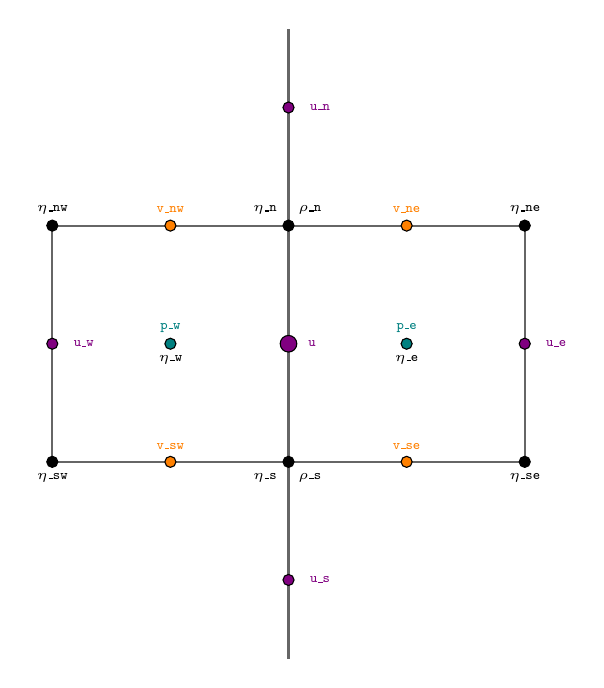
\begin{tikzpicture}
%\draw[fill=gray!23,gray!23](0,0) rectangle (8,9);
%\draw[step=0.5cm,gray,very thin] (0,0) grid (8,9); %background grid

\draw[thick,black!60] (1,3) -- (7,3) -- (7,6) -- (1,6) -- cycle ; 
\draw[thick,black!60] (4,0.5) -- (4,8.5)  ;   

%---------------------------------------------------
\node[] at (2.5,6.2) {\tiny \color{orange} \tt v\_nw};
\node[] at (2.5,3.2) {\tiny \color{orange} \tt v\_sw};
\node[] at (5.5,6.2) {\tiny \color{orange} \tt v\_ne};
\node[] at (5.5,3.2) {\tiny \color{orange} \tt v\_se};
\draw[black,fill=orange] (2.5,6)   circle (2pt);
\draw[black,fill=orange] (2.5,3)   circle (2pt);
\draw[black,fill=orange] (5.5,6)   circle (2pt);
\draw[black,fill=orange] (5.5,3)   circle (2pt);

%--------------------------------------------------
\draw[black,fill=violet] (4,1.5)   circle (2pt);
\draw[black,fill=violet] (4,4.5)   circle (3pt);
\draw[black,fill=violet] (4,7.5)   circle (2pt);
\draw[black,fill=violet] (1,4.5)   circle (2pt);
\draw[black,fill=violet] (7,4.5)   circle (2pt);
\node[] at (4.4,1.5) {\tiny \color{violet} \tt u\_s};
\node[] at (4.3,4.5) {\tiny \color{violet} \tt u};
\node[] at (4.4,7.5) {\tiny \color{violet} \tt u\_n};
\node[] at (1.4,4.5) {\tiny \color{violet} \tt u\_w};
\node[] at (7.4,4.5) {\tiny \color{violet} \tt u\_e};

\draw[black,fill=black] (1,3)   circle (2pt); 
\draw[black,fill=black] (4,3)   circle (2pt); 
\draw[black,fill=black] (7,3)   circle (2pt); 
\draw[black,fill=black] (1,6)   circle (2pt); 
\draw[black,fill=black] (4,6)   circle (2pt); 
\draw[black,fill=black] (7,6)   circle (2pt); 

%------------------------------------------------
\draw[black,fill=teal] (2.5,4.5)   circle (2pt);
\draw[black,fill=teal] (5.5,4.5)   circle (2pt);
\node[] at (2.5,4.7) {\tiny \color{teal} \tt p\_w};
\node[] at (5.5,4.7) {\tiny \color{teal} \tt p\_e};

\node[] at (4.27,2.8) {\tiny \tt $\rho$\_s};
\node[] at (4.27,6.2) {\tiny \tt $\rho$\_n};
\node[] at (2.5,4.3) {\tiny \tt $\eta$\_w};
\node[] at (5.5,4.3) {\tiny \tt $\eta$\_e};
\node[] at (3.7,2.8) {\tiny \tt $\eta$\_s};
\node[] at (3.7,6.2) {\tiny \tt $\eta$\_n};
\node[] at (7,6.2) {\tiny \tt $\eta$\_{ne}};
\node[] at (1,6.2) {\tiny \tt $\eta$\_{nw}};
\node[] at (7,2.8) {\tiny \tt $\eta$\_{se}};
\node[] at (1,2.8) {\tiny \tt $\eta$\_{sw}};
\end{tikzpicture}
\end{center}



\columnbreak

\begin{flushright} {\tiny {\color{gray} (tikz\_staggered2D\_v.tex)}} \end{flushright}
%~~~~~~~~~~~~~~~~~~~~~~~~~~~~~~~~~~~~~~~~~~~~~~~~~~~~~~~~~~~~~~~~~~~~~~~~~~~~~~~~~~~~~~~~~~~~~~~~~~



\begin{center}
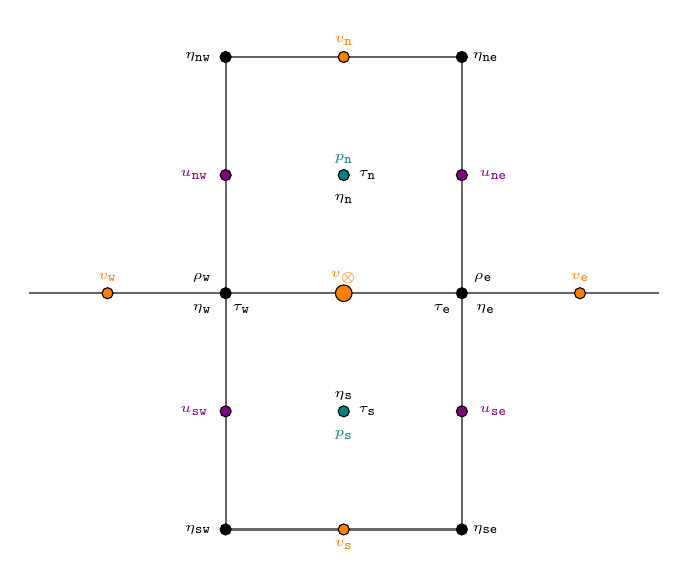
\begin{tikzpicture}
%\draw[fill=gray!23,gray!23](0,0) rectangle (9,8);
%\draw[step=0.5cm,gray,very thin] (0,0) grid (9,8); %background grid
\draw[thick,black!60] (3,1) -- (3,7) -- (6,7) -- (6,1) -- cycle ; 
\draw[thick,black!60] (0.5,4) -- (8.5,4)  ;   
%---------------------------------------------------
\node[] at (4.5,.8) {\tiny \color{orange} $v_{\tt s}$};
\node[] at (4.5,7.2) {\tiny \color{orange} $v_{\tt n}$};
\node[] at (4.5,4.2) {\tiny \color{orange} $v_\otimes$};
\node[] at (1.5,4.2) {\tiny \color{orange} $v_{\tt w}$};
\node[] at (7.5,4.2) {\tiny \color{orange} $v_{\tt e}$};
\draw[black,fill=orange] (4.5,1)   circle (2pt);
\draw[black,fill=orange] (4.5,4)   circle (3pt);
\draw[black,fill=orange] (4.5,7)   circle (2pt);
\draw[black,fill=orange] (1.5,4)   circle (2pt);
\draw[black,fill=orange] (7.5,4)   circle (2pt);
%--------------------------------------------------
\draw[black,fill=violet] (3,2.5)   circle (2pt);
\draw[black,fill=violet] (6,2.5)   circle (2pt);
\draw[black,fill=violet] (3,5.5)   circle (2pt);
\draw[black,fill=violet] (6,5.5)   circle (2pt);
\node[] at (2.6,2.5) {\tiny \color{violet} $u_{\tt sw}$};
\node[] at (6.4,2.5) {\tiny \color{violet} $u_{\tt se}$};
\node[] at (2.6,5.5) {\tiny \color{violet} $u_{\tt nw}$};
\node[] at (6.4,5.5) {\tiny \color{violet} $u_{\tt ne}$};
%-----------------------------------------------
\draw[black,fill=black] (3,1)   circle (2pt); 
\draw[black,fill=black] (3,4)   circle (2pt); 
\draw[black,fill=black] (3,7)   circle (2pt); 
\draw[black,fill=black] (6,1)   circle (2pt); 
\draw[black,fill=black] (6,4)   circle (2pt); 
\draw[black,fill=black] (6,7)   circle (2pt); 
%------------------------------------------------
\draw[black,fill=teal] (4.5,2.5)   circle (2pt);
\draw[black,fill=teal] (4.5,5.5)   circle (2pt);
\node[] at (4.5,2.2) {\tiny \color{teal} $p_{\tt s}$};
\node[] at (4.5,5.7) {\tiny \color{teal} $p_{\tt n}$};
%-----------------------------------------
\node[] at (6.27,4.2) {\tiny $\rho_{\tt e}$};
\node[] at (2.7,4.2) {\tiny $\rho_{\tt w}$};
\node[] at (4.5,5.2) {\tiny $\eta_{\tt n}$};
\node[] at (4.5,2.7) {\tiny $\eta_{\tt s}$};
\node[] at (6.3,1) {\tiny $\eta_{\tt se}$};
\node[] at (2.65,1) {\tiny $\eta_{\tt sw}$};
\node[] at (6.3,7) {\tiny $\eta_{\tt ne}$};
\node[] at (2.65,7) {\tiny $\eta_{\tt nw}$};
\node[] at (6.3,3.8) {\tiny $\eta_{\tt e}$};
\node[] at (2.7,3.8) {\tiny $\eta_{\tt w}$};

\node[] at (3.2,3.8) {\tiny $\tau_{\tt w}$};
\node[] at (5.75,3.8) {\tiny $\tau_{\tt e}$};
\node[] at (4.8,5.5) {\tiny $\tau_{\tt n}$};
\node[] at (4.8,2.5) {\tiny $\tau_{\tt s}$};


\end{tikzpicture}
\end{center}



\end{multicols}

On the left side, we see that it would be trivial to compute $\partial u/\partial x$
and $\partial u/\partial y$ on node ${\color{violet} u_\otimes}$:
\begin{eqnarray}
\frac{\partial u}{\partial x} |_{\color{violet}\otimes}
&\simeq&  \frac{ {\color{violet} u_e}-{\color{violet} u_w}  }{2h_x} \nn\\
\frac{\partial u}{\partial y} |_{\color{violet}\otimes}
&\simeq&  \frac{ {\color{violet} u_n}-{\color{violet} u_s}  }{2h_y} \nn
\end{eqnarray}
Likewise, on the right we could easily compute
\begin{eqnarray}
\frac{\partial v}{\partial x} |_{\color{orange}\otimes}
&\simeq&  \frac{ {\color{orange} v_e}-{\color{orange} v_w}  }{2h_x} \nn\\
\frac{\partial v}{\partial y} |_{\color{orange}\otimes}
&\simeq&  \frac{ {\color{orange} v_n}-{\color{orange} v_s}  }{2h_y} \nn
\end{eqnarray}
Conversely, on the left side it would be difficult to 
compute any $v$ derivative because no horizontal or vertical 
line passing by the $u$ node in the middle intersects with a 
$v$ node, and vice versa on the right side. 

It then looks like our best option to compute $\dot{\varepsilon}_{xy}$
terms is actually on the background (black) nodes since 
on the left we would have
\[
\dot{\varepsilon}_{xy}|_{\tt n} 
= 
\frac12 \left(  
\frac{\partial u}{\partial y}|_{\tt n}
+
\frac{\partial v}{\partial x}|_{\tt n}
\right)
\simeq 
\frac12 
\left( 
\frac{{\color{violet}u_{\tt n}} -{\color{violet}u_\otimes}}{h_y} + 
\frac{{\color{orange}v_{\tt ne}}-{\color{orange}u_{\tt nw}}}{h_x} 
\right)
\]
This is indeed what we find in Gerya's book at p.~137:
\begin{center}
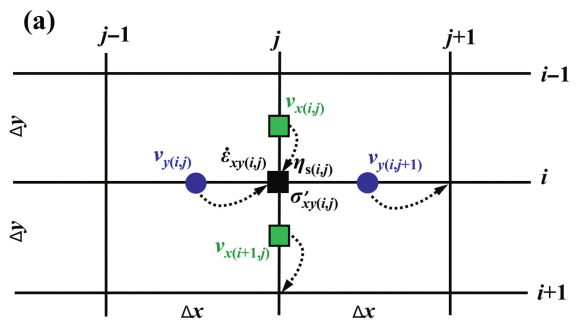
\includegraphics[width=6cm]{images/fdm/gerya_H}\\
{\captionfont Taken from Gerya (2019).}
\end{center}
However, we need to be careful with those nodes on the boundary, and
even more careful with those at the corners of the domain. 

Let us look again at our prototype mesh:

\begin{flushright} {\tiny {\color{gray} (tikz\_staggered2D\_4x3.tex)}} \end{flushright}
%~~~~~~~~~~~~~~~~~~~~~~~~~~~~~~~~~~~~~~~~~~~~~~~~~~~~~~~~~~~~~~~~~~~~~~~~~~~~~~~~~~~~~~~~~~~~~~~~~~


\begin{center}
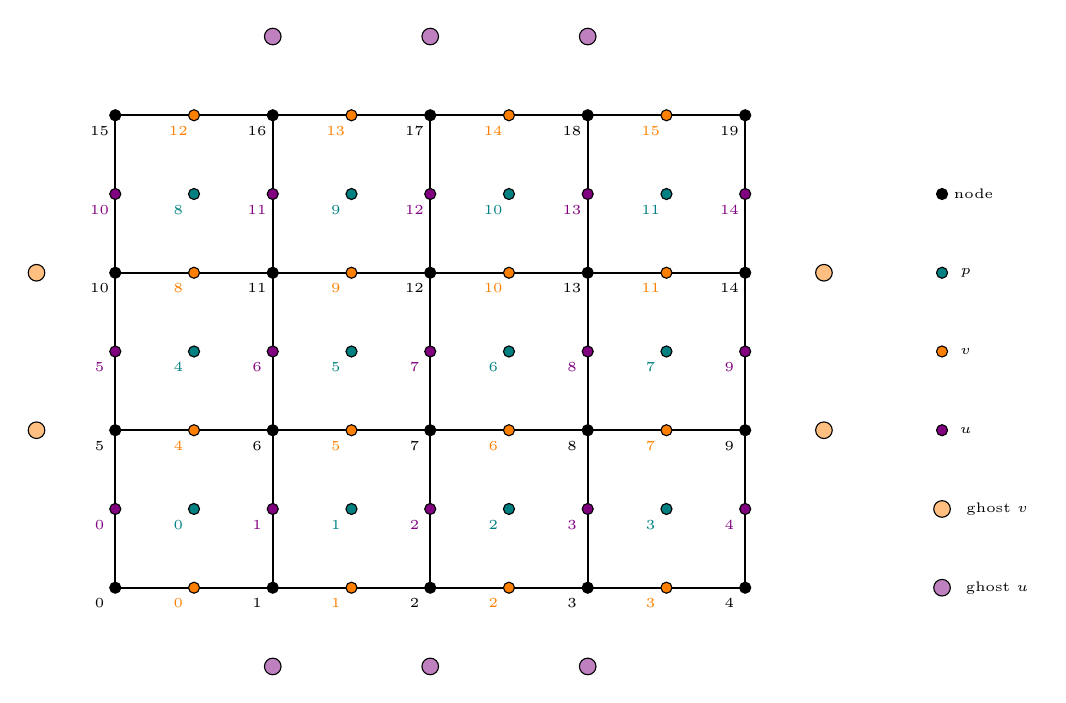
\begin{tikzpicture}
%\draw[fill=gray!23,gray!23](0,0) rectangle (12,10);
%\draw[step=0.5cm,gray,very thin] (0,0) grid (12,10); %background grid

\draw[thick] (0,0) -- (8,0) -- (8,6) -- (0,6) -- cycle ; %1-4
\draw[thick] (0,2) -- (8,2)  ; 
\draw[thick] (0,4) -- (8,4)  ; 
\draw[thick] (2,0) -- (2,6)  ; 
\draw[thick] (4,0) -- (4,6)  ; 
\draw[thick] (6,0) -- (6,6)  ; 

%pressure nodes
\draw[black,fill=teal] (1,1)   circle (2pt); 
\draw[black,fill=teal] (3,1)   circle (2pt); 
\draw[black,fill=teal] (5,1)   circle (2pt); 
\draw[black,fill=teal] (7,1)   circle (2pt); 

\draw[black,fill=teal] (1,3)   circle (2pt); 
\draw[black,fill=teal] (3,3)   circle (2pt); 
\draw[black,fill=teal] (5,3)   circle (2pt); 
\draw[black,fill=teal] (7,3)   circle (2pt); 

\draw[black,fill=teal] (1,5)   circle (2pt); 
\draw[black,fill=teal] (3,5)   circle (2pt); 
\draw[black,fill=teal] (5,5)   circle (2pt); 
\draw[black,fill=teal] (7,5)   circle (2pt); 

\node[] at (0.8,0.8) {\tiny \color{teal} 0};
\node[] at (2.8,0.8) {\tiny \color{teal} 1};
\node[] at (4.8,0.8) {\tiny \color{teal} 2};
\node[] at (6.8,0.8) {\tiny \color{teal} 3};

\node[] at (0.8,2.8) {\tiny \color{teal} 4};
\node[] at (2.8,2.8) {\tiny \color{teal} 5};
\node[] at (4.8,2.8) {\tiny \color{teal} 6};
\node[] at (6.8,2.8) {\tiny \color{teal} 7};

\node[] at (0.8,4.8) {\tiny \color{teal} 8};
\node[] at (2.8,4.8) {\tiny \color{teal} 9};
\node[] at (4.8,4.8) {\tiny \color{teal} 10};
\node[] at (6.8,4.8) {\tiny \color{teal} 11};

% u nodes
\draw[black,fill=violet] (0,1)   circle (2pt); 
\draw[black,fill=violet] (2,1)   circle (2pt); 
\draw[black,fill=violet] (4,1)   circle (2pt); 
\draw[black,fill=violet] (6,1)   circle (2pt); 
\draw[black,fill=violet] (8,1)   circle (2pt); 

\draw[black,fill=violet] (0,3)   circle (2pt); 
\draw[black,fill=violet] (2,3)   circle (2pt); 
\draw[black,fill=violet] (4,3)   circle (2pt); 
\draw[black,fill=violet] (6,3)   circle (2pt);
\draw[black,fill=violet] (8,3)   circle (2pt);

\draw[black,fill=violet] (0,5)   circle (2pt); 
\draw[black,fill=violet] (2,5)   circle (2pt); 
\draw[black,fill=violet] (4,5)   circle (2pt); 
\draw[black,fill=violet] (6,5)   circle (2pt);
\draw[black,fill=violet] (8,5)   circle (2pt);

\node[] at (-0.2,0.8) {\tiny \color{violet} 0};
\node[] at (1.8,0.8)  {\tiny \color{violet} 1};
\node[] at (3.8,0.8)  {\tiny \color{violet} 2};
\node[] at (5.8,0.8)  {\tiny \color{violet} 3};
\node[] at (7.8,0.8)  {\tiny \color{violet} 4};

\node[] at (-0.2,2.8) {\tiny \color{violet} 5};
\node[] at (1.8,2.8)  {\tiny \color{violet} 6};
\node[] at (3.8,2.8)  {\tiny \color{violet} 7};
\node[] at (5.8,2.8)  {\tiny \color{violet} 8};
\node[] at (7.8,2.8)  {\tiny \color{violet} 9};

\node[] at (-0.2,4.8){\tiny \color{violet} 10};
\node[] at (1.8,4.8) {\tiny \color{violet} 11};
\node[] at (3.8,4.8) {\tiny \color{violet} 12};
\node[] at (5.8,4.8) {\tiny \color{violet} 13};
\node[] at (7.8,4.8) {\tiny \color{violet} 14};

% v nodes
\draw[black,fill=orange] (1,0)   circle (2pt); 
\draw[black,fill=orange] (3,0)   circle (2pt); 
\draw[black,fill=orange] (5,0)   circle (2pt); 
\draw[black,fill=orange] (7,0)   circle (2pt); 

\draw[black,fill=orange] (1,2)   circle (2pt); 
\draw[black,fill=orange] (3,2)   circle (2pt); 
\draw[black,fill=orange] (5,2)   circle (2pt); 
\draw[black,fill=orange] (7,2)   circle (2pt); 

\draw[black,fill=orange] (1,4)   circle (2pt); 
\draw[black,fill=orange] (3,4)   circle (2pt); 
\draw[black,fill=orange] (5,4)   circle (2pt); 
\draw[black,fill=orange] (7,4)   circle (2pt); 

\draw[black,fill=orange] (1,6)   circle (2pt); 
\draw[black,fill=orange] (3,6)   circle (2pt); 
\draw[black,fill=orange] (5,6)   circle (2pt); 
\draw[black,fill=orange] (7,6)   circle (2pt); 

\node[] at (0.8,-0.2) {\tiny \color{orange} 0};
\node[] at (2.8,-0.2) {\tiny \color{orange} 1};
\node[] at (4.8,-0.2) {\tiny \color{orange} 2};
\node[] at (6.8,-0.2) {\tiny \color{orange} 3};

\node[] at (0.8,1.8) {\tiny \color{orange} 4};
\node[] at (2.8,1.8) {\tiny \color{orange} 5};
\node[] at (4.8,1.8) {\tiny \color{orange} 6};
\node[] at (6.8,1.8) {\tiny \color{orange} 7};

\node[] at (0.8,3.8) {\tiny \color{orange} 8};
\node[] at (2.8,3.8) {\tiny \color{orange} 9};
\node[] at (4.8,3.8) {\tiny \color{orange} 10};
\node[] at (6.8,3.8) {\tiny \color{orange} 11};

\node[] at (0.8,5.8) {\tiny \color{orange} 12};
\node[] at (2.8,5.8) {\tiny \color{orange} 13};
\node[] at (4.8,5.8) {\tiny \color{orange} 14};
\node[] at (6.8,5.8) {\tiny \color{orange} 15};

%------------------------------------------------

\draw[black,fill=black] (0,0)   circle (2pt); 
\draw[black,fill=black] (2,0)   circle (2pt); 
\draw[black,fill=black] (4,0)   circle (2pt); 
\draw[black,fill=black] (6,0)   circle (2pt); 
\draw[black,fill=black] (8,0)   circle (2pt); 

\draw[black,fill=black] (0,2)   circle (2pt); 
\draw[black,fill=black] (2,2)   circle (2pt); 
\draw[black,fill=black] (4,2)   circle (2pt); 
\draw[black,fill=black] (6,2)   circle (2pt); 
\draw[black,fill=black] (8,2)   circle (2pt); 

\draw[black,fill=black] (0,4)   circle (2pt); 
\draw[black,fill=black] (2,4)   circle (2pt); 
\draw[black,fill=black] (4,4)   circle (2pt); 
\draw[black,fill=black] (6,4)   circle (2pt); 
\draw[black,fill=black] (8,4)   circle (2pt); 

\draw[black,fill=black] (0,6)   circle (2pt); 
\draw[black,fill=black] (2,6)   circle (2pt); 
\draw[black,fill=black] (4,6)   circle (2pt); 
\draw[black,fill=black] (6,6)   circle (2pt); 
\draw[black,fill=black] (8,6)   circle (2pt); 


\node[] at (-0.2,-0.2){\tiny 0};
\node[] at (1.8,-0.2) {\tiny 1};
\node[] at (3.8,-0.2) {\tiny 2};
\node[] at (5.8,-0.2) {\tiny 3};
\node[] at (7.8,-0.2) {\tiny 4};

\node[] at (-0.2,1.8){\tiny 5};
\node[] at (1.8,1.8) {\tiny 6};
\node[] at (3.8,1.8) {\tiny 7};
\node[] at (5.8,1.8) {\tiny 8};
\node[] at (7.8,1.8) {\tiny 9};

\node[] at (-0.2,3.8){\tiny 10};
\node[] at (1.8,3.8) {\tiny 11};
\node[] at (3.8,3.8) {\tiny 12};
\node[] at (5.8,3.8) {\tiny 13};
\node[] at (7.8,3.8) {\tiny 14};

\node[] at (-0.2,5.8){\tiny 15};
\node[] at (1.8,5.8) {\tiny 16};
\node[] at (3.8,5.8) {\tiny 17};
\node[] at (5.8,5.8) {\tiny 18};
\node[] at (7.8,5.8) {\tiny 19};

%-------------------------------------------------

\draw[black,fill=black]  (10.5,5)   circle (2pt); \node[] at (10.9,5) {\tiny node};
\draw[black,fill=teal]   (10.5,4)   circle (2pt); \node[] at (10.8,4) {\tiny $p$};
\draw[black,fill=orange] (10.5,3)   circle (2pt); \node[] at (10.8,3) {\tiny $v$};
\draw[black,fill=violet] (10.5,2)   circle (2pt); \node[] at (10.8,2) {\tiny $u$};

\draw[black,fill=orange!50] (10.5,1)  circle (3pt); \node[] at (11.2,1) {\tiny ghost $v$};
\draw[black,fill=violet!50] (10.5,0)  circle (3pt); \node[] at (11.2,0) {\tiny ghost $u$};

%boundary u nodes
\draw[black,fill=violet!50] (2,-1)   circle (3pt); 
\draw[black,fill=violet!50] (4,-1)   circle (3pt); 
\draw[black,fill=violet!50] (6,-1)   circle (3pt); 
\draw[black,fill=violet!50] (2,7)   circle (3pt); 
\draw[black,fill=violet!50] (4,7)   circle (3pt); 
\draw[black,fill=violet!50] (6,7)   circle (3pt); 

%boundary u nodes
\draw[black,fill=orange!50] (-1,2)   circle (3pt); 
\draw[black,fill=orange!50] (-1,4)   circle (3pt); 
\draw[black,fill=orange!50] (9,2)   circle (3pt); 
\draw[black,fill=orange!50] (9,4)   circle (3pt); 





\end{tikzpicture}
\end{center}



Let us consider node 10. It is `missing' a left neighbour, which is 
the ghost node of ${\color{orange} v_{8}}$. 
Still operating under the assumption that boundary conditions are either 
free slip or no slip, the velocity assigned to this ghost is $\delta_{bc} {\color{orange} v_{8}}$,
so that 
\[
\dot{\varepsilon}_{xy}|_{\tt 10} 
= 
\frac12 \left(  
\frac{\partial u}{\partial y}|_{\tt 10}
+
\frac{\partial v}{\partial x}|_{\tt 10}
\right)
\simeq 
\frac12 
\left( 
\frac{{\color{violet}u_{\tt 10}} -{\color{violet}u_5}}{h_y} + 
\frac{{\color{orange}v_{\tt 8}}- \delta_{bc}{\color{orange}u_{\tt 8}}}{h_x} 
\right)
\]
Likewise, for node 3, we see that the ghost node of ${\color{violet} v_3}$
will be needed:
\[
\dot{\varepsilon}_{xy}|_{\tt 3} 
= 
\frac12 \left(  
\frac{\partial u}{\partial y}|_{\tt 3}
+
\frac{\partial v}{\partial x}|_{\tt 3}
\right)
\simeq 
\frac12 
\left( 
\frac{{\color{violet}u_{\tt 3}} -\delta_{bc} {\color{violet}u_{\tt 3}}}{h_y} + 
\frac{{\color{orange}v_{\tt 3}}- {\color{orange}u_{\tt 2}}}{h_x} 
\right)
\]
As for the corners, let us consider node 15. 
We would need the ghost node of ${\color{orange} v_{\tt 12}}$, but since 
it would be on the top boundary its $v$ value would also be zero. 
Likewise we would need the ghost node of ${\color{violet} u_{\tt 10}}$
but it would be on the left boundary so its $u$ value would be zero.
In the end we find that $\dot{\varepsilon}_{xy}=0$ in all four corners.






%------------------------------------------------------------------------
\subsection{Embedding of Particle-In-Cell}

how to interpolate fields onto particles?

section 8.4, 8.5 of book

%------------------------------------------------------------------------
\subsection{Measure errors}

TODO

%------------------------------------------------------------------------
\subsection{Non-equidistant nodes \label{ss:fdm_stokes_hvar}}

TODO

























\newpage
\begin{landscape}
{\tiny
\[
\left(
\begin{array}{c|c|c|c|c|c|c|c|c|c|c|c|c|c|c|c|c|c|c|c|c|c|c|c|c|c|c|c|c|c|c|c|c|c|c|c|c|c|c|c|c|c|c}
1 & 2 & 3 & 4 & 5 & 6 & 7 & 8 & 9 &
10 & 11 &12 &13 &14 &15& 16& 17& 18& 19 &
20 &21 &22 &23 & 24 & 25 & 26 & 27 & 28 & 29 &
30 &21 &22 &23 & 24 & 25 & 26 & 27 & 28 & 29 &
40 & 41 & 42 & 43 \\
. & . & . & . & . & . & . & . & . & . & . & . & . & . & . & . & . & . & . & . & . & . & . & . & . & 
. & . & . & . & . & . & . & . & . & . & . & . & . & . & . & . & . & . \\
. & . & . & . & . & . & . & . & . & . & . & . & . & . & . & . & . & . & . & . & . & . & . & . & . & 
. & . & . & . & . & . & . & . & . & . & . & . & . & . & . & . & . & . \\
. & . & . & . & . & . & . & . & . & . & . & . & . & . & . & . & . & . & . & . & . & . & . & . & . & 
. & . & . & . & . & . & . & . & . & . & . & . & . & . & . & . & . & . \\
. & . & . & . & . & . & . & . & . & . & . & . & . & . & . & . & . & . & . & . & . & . & . & . & . & 
. & . & . & . & . & . & . & . & . & . & . & . & . & . & . & . & . & . \\
. & . & . & . & . & . & . & . & . & . & . & . & . & . & . & . & . & . & . & . & . & . & . & . & . & 
. & . & . & . & . & . & . & . & . & . & . & . & . & . & . & . & . & . \\
. & . & . & . & . & . & . & . & . & . & . & . & . & . & . & . & . & . & . & . & . & . & . & . & . & 
. & . & . & . & . & . & . & . & . & . & . & . & . & . & . & . & . & . \\
. & . & . & . & . & . & . & . & . & . & . & . & . & . & . & . & . & . & . & . & . & . & . & . & . & 
. & . & . & . & . & . & . & . & . & . & . & . & . & . & . & . & . & . \\
. & . & . & . & . & . & . & . & . & . & . & . & . & . & . & . & . & . & . & . & . & . & . & . & . & 
. & . & . & . & . & . & . & . & . & . & . & . & . & . & . & . & . & . \\
. & . & . & . & . & . & . & . & . & . & . & . & . & . & . & . & . & . & . & . & . & . & . & . & . & 
. & . & . & . & . & . & . & . & . & . & . & . & . & . & . & . & . & . \\
. & . & . & . & . & . & . & . & . & . & . & . & . & . & . & . & . & . & . & . & . & . & . & . & . & 
. & . & . & . & . & . & . & . & . & . & . & . & . & . & . & . & . & . \\
\hline
. & . & . & . & . & . & . & . & . & . & . & . & . & . & . & . & . & . & . & . & . & . & . & . & . & 
. & . & . & . & . & . & . & . & . & . & . & . & . & . & . & . & . & . \\
. & . & . & . & . & . & . & . & . & . & . & . & . & . & . & . & . & . & . & . & . & . & . & . & . & 
. & . & . & . & . & . & . & . & . & . & . & . & . & . & . & . & . & . \\
. & . & . & . & . & . & . & . & . & . & . & . & . & . & . & . & . & . & . & . & . & . & . & . & . & 
. & . & . & . & . & . & . & . & . & . & . & . & . & . & . & . & . & . \\
. & . & . & . & . & . & . & . & . & . & . & . & . & . & . & . & . & . & . & . & . & . & . & . & . & 
. & . & . & . & . & . & . & . & . & . & . & . & . & . & . & . & . & . \\
. & . & . & . & . & . & . & . & . & . & . & . & . & . & . & . & . & . & . & . & . & . & . & . & . & 
. & . & . & . & . & . & . & . & . & . & . & . & . & . & . & . & . & . \\
. & . & . & . & . & . & . & . & . & . & . & . & . & . & . & . & . & . & . & . & . & . & . & . & . & 
. & . & . & . & . & . & . & . & . & . & . & . & . & . & . & . & . & . \\
. & . & . & . & . & . & . & . & . & . & . & . & . & . & . & . & . & . & . & . & . & . & . & . & . & 
. & . & . & . & . & . & . & . & . & . & . & . & . & . & . & . & . & . \\
. & . & . & . & . & . & . & . & . & . & . & . & . & . & . & . & . & . & . & . & . & . & . & . & . & 
. & . & . & . & . & . & . & . & . & . & . & . & . & . & . & . & . & . \\
. & . & . & . & . & . & . & . & . & . & . & . & . & . & . & . & . & . & . & . & . & . & . & . & . & 
. & . & . & . & . & . & . & . & . & . & . & . & . & . & . & . & . & . \\
. & . & . & . & . & . & . & . & . & . & . & . & . & . & . & . & . & . & . & . & . & . & . & . & . & 
. & . & . & . & . & . & . & . & . & . & . & . & . & . & . & . & . & . \\
\hline
. & . & . & . & . & . & . & . & . & . & . & . & . & . & . & . & . & . & . & . & . & . & . & . & . & 
. & . & . & . & . & . & . & . & . & . & . & . & . & . & . & . & . & . \\
. & . & . & . & . & . & . & . & . & . & . & . & . & . & . & . & . & . & . & . & . & . & . & . & . & 
. & . & . & . & . & . & . & . & . & . & . & . & . & . & . & . & . & . \\
. & . & . & . & . & . & . & . & . & . & . & . & . & . & . & . & . & . & . & . & . & . & . & . & . & 
. & . & . & . & . & . & . & . & . & . & . & . & . & . & . & . & . & . \\
. & . & . & . & . & . & . & . & . & . & . & . & . & . & . & . & . & . & . & . & . & . & . & . & . & 
. & . & . & . & . & . & . & . & . & . & . & . & . & . & . & . & . & . \\
. & . & . & . & . & . & . & . & . & . & . & . & . & . & . & . & . & . & . & . & . & . & . & . & . & 
. & . & . & . & . & . & . & . & . & . & . & . & . & . & . & . & . & . \\
. & . & . & . & . & . & . & . & . & . & . & . & . & . & . & . & . & . & . & . & . & . & . & . & . & 
. & . & . & . & . & . & . & . & . & . & . & . & . & . & . & . & . & . \\
. & . & . & . & . & . & . & . & . & . & . & . & . & . & . & . & . & . & . & . & . & . & . & . & . & 
. & . & . & . & . & . & . & . & . & . & . & . & . & . & . & . & . & . \\
. & . & . & . & . & . & . & . & . & . & . & . & . & . & . & . & . & . & . & . & . & . & . & . & . & 
. & . & . & . & . & . & . & . & . & . & . & . & . & . & . & . & . & . \\
. & . & . & . & . & . & . & . & . & . & . & . & . & . & . & . & . & . & . & . & . & . & . & . & . & 
. & . & . & . & . & . & . & . & . & . & . & . & . & . & . & . & . & . \\
. & . & . & . & . & . & . & . & . & . & . & . & . & . & . & . & . & . & . & . & . & . & . & . & . & 
. & . & . & . & . & . & . & . & . & . & . & . & . & . & . & . & . & . \\
\hline
. & . & . & . & . & . & . & . & . & . & . & . & . & . & . & . & . & . & . & . & . & . & . & . & . & 
. & . & . & . & . & . & . & . & . & . & . & . & . & . & . & . & . & . \\
. & . & . & . & . & . & . & . & . & . & . & . & . & . & . & . & . & . & . & . & . & . & . & . & . & 
. & . & . & . & . & . & . & . & . & . & . & . & . & . & . & . & . & . \\
. & . & . & . & . & . & . & . & . & . & . & . & . & . & . & . & . & . & . & . & . & . & . & . & . & 
. & . & . & . & . & . & . & . & . & . & . & . & . & . & . & . & . & . \\
. & . & . & . & . & . & . & . & . & . & . & . & . & . & . & . & . & . & . & . & . & . & . & . & . & 
. & . & . & . & . & . & . & . & . & . & . & . & . & . & . & . & . & . \\
. & . & . & . & . & . & . & . & . & . & . & . & . & . & . & . & . & . & . & . & . & . & . & . & . & 
. & . & . & . & . & . & . & . & . & . & . & . & . & . & . & . & . & . \\
. & . & . & . & . & . & . & . & . & . & . & . & . & . & . & . & . & . & . & . & . & . & . & . & . & 
. & . & . & . & . & . & . & . & . & . & . & . & . & . & . & . & . & . \\
. & . & . & . & . & . & . & . & . & . & . & . & . & . & . & . & . & . & . & . & . & . & . & . & . & 
. & . & . & . & . & . & . & . & . & . & . & . & . & . & . & . & . & . \\
. & . & . & . & . & . & . & . & . & . & . & . & . & . & . & . & . & . & . & . & . & . & . & . & . & 
. & . & . & . & . & . & . & . & . & . & . & . & . & . & . & . & . & . \\
. & . & . & . & . & . & . & . & . & . & . & . & . & . & . & . & . & . & . & . & . & . & . & . & . & 
. & . & . & . & . & . & . & . & . & . & . & . & . & . & . & . & . & . \\
. & . & . & . & . & . & . & . & . & . & . & . & . & . & . & . & . & . & . & . & . & . & . & . & . & 
. & . & . & . & . & . & . & . & . & . & . & . & . & . & . & . & . & . \\
\hline
. & . & . & . & . & . & . & . & . & . & . & . & . & . & . & . & . & . & . & . & . & . & . & . & . & 
. & . & . & . & . & . & . & . & . & . & . & . & . & . & . & . & . & . \\
. & . & . & . & . & . & . & . & . & . & . & . & . & . & . & . & . & . & . & . & . & . & . & . & . & 
. & . & . & . & . & . & . & . & . & . & . & . & . & . & . & . & . & . \\
. & . & . & . & . & . & . & . & . & . & . & . & . & . & . & . & . & . & . & . & . & . & . & . & . & 
. & . & . & . & . & . & . & . & . & . & . & . & . & . & . & . & . & . 
\end{array}
\right)
%\cdot
%\vec{X}=
%\left(
%\begin{array}{c}
%0 \\ . \\ . \\ 0 \\ 0 \\ . \\ . \\ 0 \\
%X \\
%0 \\ 0 \\ 0 \\ 0\\ 0 \\ 0
%\end{array}
%\right)
\]
}
\end{landscape}

